\documentclass[11pt,a4paper]{article}
\usepackage[utf8]{inputenc}
\usepackage[dvipsnames]{xcolor}
\usepackage[english]{babel}
\usepackage{listings}
\usepackage{multirow}
\usepackage{color}
\usepackage[hidelinks]{hyperref}
\usepackage[ruled,vlined]{algorithm2e}
\renewcommand*{\thefootnote}{\fnsymbol{footnote}}
\usepackage{mathrsfs}
\usepackage{hyperref}
\usepackage{adjustbox} %adjust boxe til den rigtige størrelse
 \usepackage{biblatex} %Imports biblatex package
\addbibresource{sample.bib} %Import the bibliography file
\appto{\bibsetup}{\raggedright}

\lstset{ %
  language=R,                     % the language of the code
  basicstyle=\footnotesize,       % the size of the fonts that are used for the code
  numbers=left,                   % where to put the line-numbers
  numberstyle=\tiny\color{gray},  % the style that is used for the line-numbers
  stepnumber=1,                   % the step between two line-numbers. If it's 1, each line
                                  % will be numbered
  numbersep=5pt,                  % how far the line-numbers are from the code
  backgroundcolor=\color{white},  % choose the background color. You must add \usepackage{color}
  showspaces=false,               % show spaces adding particular underscores
  showstringspaces=false,         % underline spaces within strings
  showtabs=false,                 % show tabs within strings adding particular underscores
  frame=single,                   % adds a frame around the codehttps://da.overleaf.com/project/5e42ac84ac4e640001f94558
  rulecolor=\color{black},        % if not set, the frame-color may be changed on line-breaks within not-black text (e.g. commens (green here))
  tabsize=2,                      % sets default tabsize to 2 spaces
  captionpos=b,                   % sets the caption-position to bottom
  breaklines=true,                % sets automatic line breaking
  breakatwhitespace=false,        % sets if automatic breaks should only happen at whitespace
  title=\lstname,                 % show the filename of files included with \lstinputlisting;
                                  % also try caption instead of title
  keywordstyle=\color{blue},      % keyword style
  commentstyle=\color{ForestGreen},   % comment style
  stringstyle=\color{mauve},      % string literal style
  escapeinside={\%*}{*)},         % if you want to add a comment within your code
  morekeywords={*,...}            % if you want to add more keywords to the set
}
\usepackage{amsmath}
\DeclareMathOperator{\sgn}{sgn}
\usepackage{graphicx}
\usepackage{capt-of}
\usepackage{import}
\usepackage{booktabs, array}
\usepackage{siunitx}
\usepackage{tabularx}
\usepackage{dcolumn}
\usepackage{longtable}
\usepackage{amssymb}
\usepackage{arydshln}
\usepackage{titlesec}
\graphicspath{ {pictures/} }
\addto\captionsenglish{
    \renewcommand*\contentsname{Table of Contents}
}
\usepackage{caption}
\captionsetup[figure]{labelfont=Large}
\captionsetup[table]{labelfont=Large}
\addto\captionsenglish{%
  \renewcommand{\figurename}{Figur}%
  \renewcommand{\tablename}{Tabel}%
}
\usepackage{graphicx}
\usepackage{subcaption}
\usepackage{cleveref}
\captionsetup[subfigure]{subrefformat=simple,labelformat=simple}
\renewcommand\thesubfigure{(\alph{subfigure})}
\usepackage{wrapfig}
\usepackage{lineno, blindtext}
\usepackage{helvet}
\usepackage{longtable}
\usepackage{fullpage}
\def\DU#1{\underline{\underline{#1}}}
\def\SU#1{\underline{#1}}
\definecolor{mygreen}{rgb}{0,0.6,0}
\usepackage{listings}
\usepackage{ulem}
\begin{document}
\begin{titlepage} % Suppresses displaying the page number on the title page and the subsequent page counts as page 1
	\newcommand{\HRule}{\rule{\linewidth}{0.5mm}} % Defines a new command for horizontal lines, change thickness here
	
	\center % Centre everything on the page
	
	%------------------------------------------------
	%	Headings
	%------------------------------------------------
	
	\textsc{\LARGE Copenhagen Business School}\\[1.5cm] % Main heading such as the name of your university/college
	
	\textsc{\Large Statistik}\\[0.5cm] % Major heading such as course name
	
	\textsc{\large Bachelorprojekt}\\[0.5cm] % Minor heading such as course title
	
	%------------------------------------------------
	%	Title
	%------------------------------------------------
	
	\HRule\\[0.4cm]
	
	{\huge\bfseries Implementering af Rao-Kupper modellen med parameteroptimering og -udvælgelse ved brug af lasso}\\[0.4cm] % Title of your document
	
	\HRule\\[1.5cm]
	
	%------------------------------------------------
	%	Author(s)
	%------------------------------------------------
	
	\begin{minipage}{0.4\textwidth}
		\begin{flushleft}
			\large
			\textit{Forfattere}\\
			Lucas Johan Boesen\\ % Your name
			Christoffer Bolvig Birch\\ % Your name
			Victor Emil Skov Lundmark\\ % Your name
		\end{flushleft}
	\end{minipage}
	~
	\begin{minipage}{0.4\textwidth}
		\begin{flushright}
			\large
			\textit{Professor}\\
			\textsc{Søren Feodor Nielsen}\\
			\textsc{}\\
			\textsc{}\\% Supervisor's name
		\end{flushright}
	\end{minipage}
	
	% If you don't want a supervisor, uncomment the two lines below and comment the code above
	%{\large\textit{Author}}\\
	%John \textsc{Smith} % Your name
	
	%------------------------------------------------
	%	Date
	%------------------------------------------------
	
	\vfill\vfill\vfill % Position the date 3/4 down the remaining page
	
	{\large{25 maj 2020}} % Date, change the \today to a set date if you want to be precise
	
	%------------------------------------------------
	%	Logo
	%------------------------------------------------
	
	%\vfill\vfill
	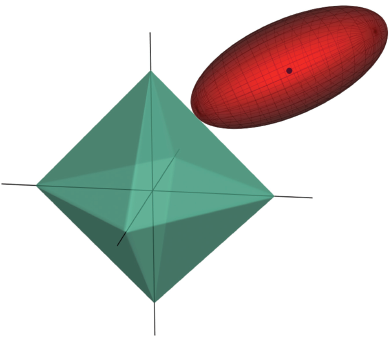
\includegraphics[width=0.7 \textwidth]{GLR2.png}\\[1cm]% Include a department/university logo - this will require the graphicx package
	 
	%----------------------------------------------------------------------------------------
	
	\vfill % Push the date up 1/4 of the remaining page
	
\end{titlepage}
\begin{abstract}
In a model for ranking products based on paired comparisons, the probability of product $i$ being preferred to product $j$ is a function of their relative strengths. Our first purpose is to show how the model is generalized to include the outcome tie and how the lasso method can be used to selecting important parameters. Our second and more specific purpose is to implement a suitable code to test the model on ranking football teams and predicting the outcome of football matches in the danish \textit{Superliga}.\newline\newline
\textit{Key words: }\;\;\; Bradley-Terry model, Rao-Kupper model, Lasso, rank analysis, sports predicting. 
\end{abstract}
\clearpage
\renewcommand{\contentsname}{Indhold}
\clearpage
\tableofcontents
\clearpage
\newpage
\pagenumbering{arabic}
\#TODOLIST
Abstract\\
Konklusion\\
Indledning\\
evt kød på diskussion\\
\sout{Fix Plots}\\
\sout{Plots af forskel i odds} \\
Tjek alle ligninger \\
\sout{Opdater styrker og betaer i tabel}\\
\sout{Beregn styrker for lasso modeller} \\
Preface \\
Tjek efter blå textrettelser \\
\sout{Standardfejl i lasso} \\

\section{Indledning}
Rangeringer af grupper spiller en stor rolle i vores samfund, det bliver først og fremmest brugt i konkurrencer, men også indirekte hver gang vi foretager et valg med flere muligheder. Hver gang vi handler ind, skal vi foretage et valg mellem forskellige produkter, hvilket ender ud i at vi foretrækker ét produkt over et andet/de andre mulige produkter. Til at beskrive disse rangeringer foreslog Bradley og Terry (1952) \cite{BradleyTerry}, en model til at rangere grupper ud fra parvise sammenligninger, hvor der for hver sammenligning altid vil være et foretrukket valg. Denne model er en grundsten i mange rangeringssystemer, eksempelvis ELO-rating som bliver anvendt til at rangere skakspillere. At spørge en forbruger om at rangere to produkter ad gangen, fremfor at rangere en hel gruppe simultant, er i praksis en mere håndterbar metode, ikke mindst fordi det efterlader forbrugeren med et mindre udfaldsrum.\\
At der altid i parvise sammenligninger kun vil være to mulige udfald, er dog ikke en generel nok antagelse; ofte vil der være situationer hvor der ikke kan træffes ét klart foretrukket valg. Til at beskrive disse situationer har Rao og Kupper (1967) \cite{RaoKupper} videreudviklet modellen, til at kunne beskrive parvise sammenligninger med tre udfald, hvilket åbner op for, at vi kan rangere langt flere grupper. Metoden til at rangere grupperne, bygger på at der estimeres styrker for hvert element i gruppen, ud fra udfaldene af forrige sammenligninger i gruppen. Udfaldende for de parvise sammenligninger, kan ved hjælp af styrkerne oversættes til sandsynligheder, for hvad fremtidige udfald af parvise sammenligninger vil blive. Det sidste er i tilfælde hvor man allerede har defineret et klart rangeringssystem, som i sports verdenen, det mest spændende at gå i dybden med. Af denne årsag vil vi i denne rapport redegøre for og implementere Rao og Kuppers model i \textit{R} på to forskellige måder; en til rangering og en til forudsigelse. I mangel af bedre ord, har vi i rapporten valgt at omtale anvendelserne af Rao og Kuppers model som henholdsvis "Rao-Kupper" og "den dynamiske model" til rangering og til forudsigelse. Tanken bag er at "Rao-Kupper" \\
Et problem der kun bliver større og større i den digitale tidsalder, er den store mængde af data der er tilgængelig, og dermed problemet med hvilket datamateriale man skal anvende. Til at løse dette problem foreslog Robert Tibshirani (1992) \cite{RobertTibshirani}, en løsning; lasso. Lasso er en metode til at bestemme størrelsen samt udvælge de mest beskrivende parametre i en model, til at forbedre dens prædiktionsevne. Denne metode vil vi i opgaven anvende til at forbedre vores model.   
 \\ \newline
Rapporten er struktureret i fire hovedafsnit. Afsnit 2 beskriver teorien bag udviklingen fra Bradley-Terry modellen til Rao-Kupper modellen, og redegør for teorien bag hvordan den kan implementeres i praksis ved brug af kovariater til at estimere styrkerne. Afsnit 3 beskriver hvordan modellen skal anvendes til at rangere og hvordan den skal anvendes til at forudsige, samt hvordan den bliver implementeret og testet. Afsnit 4 forklarer idéen og teorien bag lasso, som bruges til at mindske størrelsen og udvælge de mest beskrivende parametre i modellen. Afsnit 5 indeholder resultater fra implementeringen af lasso og afsluttende bemærkninger om hvordan lasso har influeret modellen.

grupper er svært men par er nemt. 
\subsection{Problemformulering}
Hvordan kan Rao-Kuppers generalisering af Bradley-Terry modellen anvendes til bestemmelse af sandsynligheder ud fra parvise sammenligninger i situationer med tre udfald, og hvordan kan Lasso anvendes til at forbedre denne? Hvordan kan modellen implementeres og anvendes i praksis til at estimere sandsynligheder for udfald af fodboldkampe i superligaen? 
\subsection{Afgrænsning}
Rapporten fokuserer på hvordan det er muligt at rangere grupper ud fra parvise sammenligninger, 
Start med hvad vi har gjort og slut med hvad vi ikke har gjort. 

Det er dog ikke gjort i dette projekt, eftersom vi har valgt at fokusere på hvordan modellen kan anvendes med data, hvormed vi har prøvet
\section{Generalisering af Bradley-Terry modellen}
I dette afsnit præsenterer vi, hvordan vi tolker Bradley-Terry modellen, hvordan vi bruger modellen til at lave parvise sammenligninger, samt hvordan vi estimerer modellens parametre.\\ \newline
Bradley og Terry (1952)\cite{BradleyTerry} introducerer en statistisk model til rangering, af eksempelvis forbrugervurderinger af produkter eller styrker af fodboldhold, ved parvise sammenligninger. Dette gøres ved at estimere nytter for produkterne eller styrker af fodboldholdene. I førstnævnte eksempel vil modellen yderligere kunne bruges til at estimere sandsynligheden for, at en forbruger foretrækker ét produkt over et andet - i sidstnævnte eksempel til at estimere sandsynligheden for, at BIF vinder over FCK i deres næste opgør.\\ I dette projekt tager vi udgangspunkt i eksemplet med sammenligninger af fodboldhold og når vi i løbet af projektet beskriver parvise sammenligninger, vil vi altid tage udgangspunkt i sammenligningen af hold $i$ med hold $j$, hvor $i<j$. Vi lader \\$i \in \{1,..,h-1\}$ og $j\in \{i+1,...,h\}$ hvor $h\in \mathbb{Z}^+$ er antal fodboldhold der sammenlignes. På denne måde undgår vi at gentage parvise sammenligninger af hold \textit{i} og hold \textit{j}, samt at sammenligne hold med sig selv. 
\subsection{Bradley-Terry modellen}
Modellen som Bradley og Terry (1952)\cite{BradleyTerry} foreslog skriver vi som:
\begin{align*}
    P(i\ vinder\ over\ j) = p_{i\cdot ij} = \frac{\pi_i}{\pi_i+\pi_j},
\end{align*}
\\
hvor $p_{i\cdot ij}$ er sandsynligheden for at hold \textit{i} vinder over hold \textit{j}. Vi tolker $\pi_i>0$ og $\pi_j>0$ som hold \textit{i} og \textit{j}'s respektive styrker, og lader $Y_i=\pi_i+\epsilon_i$ betegne hold \textit{i}'s dagsform. Dette medfører hold \textit{i} vinder over hold \textit{j}, hvis $Y_i>Y_j$. 
Eftersom modellens parametre kan skaleres op uden at det påvirker sandsynlighederne:
\begin{align*}
p_{i\cdot ij} = \frac{\pi_i}{\pi_i+\pi_j} = \frac{\pi_iC}{\pi_iC+\pi_jC},
\end{align*}
ses modellen at være overparameteriseret. Det er dermed ikke muligt at identificere de enkelte styrkeparametre, men det er muligt at identificere forholdet mellem to styrkeparametre. Det problem klarer vi ved, at sætte et af holdenens styrker fast, for så at estimere de andre holds styrker relativt til holdet med fast styrke.\\
Ved omskrivning af $p_{i\cdot ij}$ udtrykker vi dette styrkeforhold som:
\begin{align*}
    p_{i\cdot ij} &= \frac{\pi_i}{\pi_i+\pi_j}=\frac{1}{1+\frac{\pi_j}{\pi_i}}=\frac{1}{1+e^{-(\log(\pi_i)-\log(\pi_j))}}\\
    &=F(V_{i\cdot ij})=\int_{-\infty}^{V_{i\cdot ij}} \frac{\partial p_{i\cdot ij}}{\partial V_{i\cdot ij}} \text{ d}V=\frac{1}{1+e^{-V_{i\cdot ij}}},
\end{align*}
hvor $V_{i\cdot ij}=\log(\pi_i)-\log(\pi_j)$ beskriver log-styrken for hold \textit{i} i forhold til hold \textit{j}. Vi ser at sandsynligheden for at hold \textit{i} vinder over hold \textit{j} er bestemt ved forskellen i log-styrker for de to hold. Eftersom 
\begin{align*}
&f(V_{i\cdot ij})=\frac{\partial p_{i\cdot ij}}{\partial V_{i\cdot ij}} = \frac{e^{-V_{i\cdot ij}}}{(e^{-V_{i\cdot ij}}+1)^2} \geq 0, \\ 
\intertext{samt at}
&\int_{-\infty}^\infty f(V_{i\cdot ij}) \text{  d} V_{i\cdot ij} = 1,
\end{align*}
er $f(V_{i\cdot ij})$ en tæthed for den logistiske fordeling, hvor $F(V_{i\cdot ij})$ er den tilhørende fordelingsfunktion, som for givne styrke parametre, kan opfattes som en sandsynlighed.\\
Sandsynligheden for, at hold \textit{i} vinder over hold \textit{j} på en given kampdag, kan dermed tolkes som sandsynligheden for at hold \textit{i}'s dagsform er bedre (større) end hold \textit{j}'s:
\begin{align*}
p_{i\cdot ij}&=P\big{\{}Y_i>Y_j\big{\}}
\\&=P\big{\{}(\pi_i-\pi_j)+(\epsilon_i-\epsilon_j)>0\big{\}}
\\&=P\big{\{}(\epsilon_i-\epsilon_j)>(\pi_j-\pi_i)\big{\}}
\\&=\frac{1}{1+e^{-(log(\pi_i)-log(\pi_j))}} 
\\&=\frac{\pi_i}{\pi_i+\pi_j}.\;\;
\end{align*}
\\
Vi antager, at $\epsilon_i$'erne er uafhængige og gumbelfordelte, fordi det medfører at forskellen $\epsilon_i-\epsilon_j$ er logistisk fordelt, hvilket giver anledning til at bruge den logistiske linkfunktion.
\subsection{Rao-Kupper modellen}
Indtil videre har vi antaget at en fodboldkamp altid har haft en vinder, men dette er ikke en realistisk antagelse, da fodboldkampe kan ende uafgjort. Det samme gælder forbrugerpræferencen mellem to produkter. Realistisk set, kan en forbruger være ligeglad ved valget mellem to produkter, hvis produkterne giver forbrugeren tilnærmelsesvist den samme nytte. Rao og Kupper (1967) \cite{RaoKupper} foreslår en løsning på dette dilemma; at udvide Bradley-Terry modellen med en grænseværdiparameter $\theta$. $\theta$ betegner den forskel i dagsform der mindst skal være mellem to hold, for at der er en vinder; hvis $\|Y_i-Y_j\| < \theta$ bliver kampen uafgjort. Rao-Kupper opskrives som integralet af en tæthed ligesom Bradley-Terry, og giver sandsynlighederne:
\begin{equation}
\begin{split}
    p_{i\cdot ij}&=F(V_{i\cdot ij}-\eta)=\frac{\pi_i}{\pi_i+\theta \pi_j}\\
    p_{j\cdot ij}&=F(V_{j\cdot ij}-\eta)=1-F(V_{i\cdot ij}+\eta)=\frac{\pi_j}{\theta \pi_i+\pi_j}\\
    p_{0\cdot ij}&=F(V_{i\cdot ij}+\eta)-F(V_{i\cdot ij}-\eta)= \frac{\pi_i \pi_j(\theta^2 -1)}{(\pi_i+\theta \pi_j)(\theta \pi_i + \pi_j)} \label{Sandynligheder},
\end{split}
\end{equation}
hvor $\eta=\log(\theta)>0 \rightarrow\theta>1$ og $p_{0\cdot ij}$ er sandsynligheden for det nye udfald, uafgjort. Sandsynlighederne er direkte sammenlignelige med et rangeringssystem, hvor hvert udfald giver en forskellig rangering mellem de to hold. I fodbold får vinderholdet 3 point, taberholdet 0 point og hvis kampen ender uafgjort får begge hold 1 point. Ligeledes vil en forbruger der står overfor valget mellem to produkter, enten synes det ene produkt er bedre, dårligere eller lige så godt som det andet.
\subsection{Parameterestimering}
I dette underafsnit viser vi en måde at estimere \textit{maximum likelihood} estimaterne for parametrene i Rao-Kupper modellen og deres tilhørende fordeling.
Rao-Kupper modellen er en delmodel af den almindelige multinomialfordelingsmodel, som vi vil tage udgangspunkt i, når vi opstiller likelihooden.\\
Lad $y_{ij}(t)$ være en tredimensionel uafhængig stokastisk variabel, som repræsenterer en kamp mellem hold \textit{i} og hold \textit{j} til tidspunkt $t$. $y_{ij}(t)$'s, tilhørende udfaldsområde er dermed givet ved 0-1 variablene $\big{(}y_{i\cdot ij}(t),\;y_{j\cdot ij}(t),\;y_{0\cdot ij}(t)\big{)}$, som hhv. repræsenterer sejr til hold \textit{i}, sejr til hold \textit{j} og uafgjort: 
\begin{align*}
  y_{i\cdot ij}(t)&=\begin{cases}
1\text{, hvis hold $i$ vinder over hold $j$ til tidspunkt $t$}\\
0\text{, ellers}
\end{cases},\\
 y_{j\cdot ij}(t)&=\begin{cases}
1\text{, hvis hold $j$ vinder over hold $i$ til tidspunkt $t$}\\
0\text{, ellers}
\end{cases},\\
 y_{0\cdot ij}(t)&=\begin{cases}
1\text{, hvis hold $i$ og hold $j$ spiller uafgjort til tidspunkt $t$}\\
0\text{, ellers}
\end{cases},
\end{align*}
dermed bliver de tilhørende sandsynligheder:
\begin{align*}
   &P\{y_{i\cdot ij}(t)=1\}=p_{i\cdot ij} &&P\{y_{j\cdot ij}(t)=1\}=p_{j\cdot ij} &&P\{y_{0\cdot ij}(t)=1\}=p_{0\cdot ij}.
\end{align*}
 Kontingenstabellen for kampe mellem hold $i$ og hold $j$ for en given periode $t=\{1,..,n\}$ kalder vi $Y_{ij}=(Y_{i\cdot ij},Y_{j\cdot ij},Y_{0\cdot ij})$, hvor:
\begin{align*}
    &Y_{i\cdot ij}=\sum_{t=1}^{n}y_{i\cdot ij}(t) &&Y_{j\cdot ij}=\sum_{t=1}^ny_{j\cdot ij}(t) &&Y_{0\cdot ij}=\sum_{t=1}^ny_{0\cdot ij}(t)
\end{align*}
\\
Yderligere lader vi $r_{ij}(t)$ være en 0-1 variabel som beskriver, hvorvidt hold $i$ har spillet mod hold $j$ til tidspunkt $t$:
\begin{align*}
r_{ij}(t)&=\begin{cases}
1\text{, hvis hold $i$ spiller mod hold $j$ til tidspunkt $t$}\\
0\text{, ellers}
\end{cases},
\end{align*}
og lader $R_{ij}=\sum_{t=1}^nr_{ij}(t)$ være antal kampe mellem hold $i$ og hold $j$, for perioden $t=\{1,...,n\}$. $R_{ij}$ og $r_{ij}(t)$ er praktiske til at omskrive modellen, for at lette notationerne i udregningerne; $y_{0\cdot ij}(t)=r_{ij}(t)-y_{i\cdot ij}(t)-y_{j\cdot ij}(t)$ og $Y_{0\cdot ij}=R_{ij}-Y_{i\cdot ij}-Y_{j\cdot ij}$\\
Likelihood-funktionen som (Rao og Kupper 1967) \cite{RaoKupper} foreslår, skriver vi som:
\begin{align}
\mathcal{L}\big{(}\pi_1,...,\pi_h,\theta\big{)} &= \prod_{i<j}p_{i\cdot ij}^{Y_{i\cdot ij}}p_{j\cdot ij}^{Y_{j\cdot ij}}p_{0\cdot ij}^{Y_{0\cdot ij}}  \nonumber\\
&= \prod_{i<j}\Big{(}\frac{\pi_i}{\pi_i+\theta\pi_j}\Big{)}^{Y_{i\cdot ij}} \label{func:LikelihoodUdenBeta}
\;\Big{(}\frac{\pi_j}{\pi_j+\theta\pi_i}\Big{)}^{Y_{j\cdot ij}}
\Big{(}\frac{(\theta^2-1)\pi_i \pi_j}{(\pi_i+\theta\pi_j)(\pi_j+\theta\pi_i)}\Big{)}^{Y_{0\cdot ij}}\\
&=\prod_{i<j}\Big{(}\frac{\pi_i}{\pi_i+\theta\pi_j}\Big{)}^{Y_{i\cdot ij}}
\;\Big{(}\frac{\pi_j}{\pi_j+\theta\pi_i}\Big{)}^{Y_{j\cdot ij}}
\Big{(}\frac{(\theta^2-1)\pi_i  \pi_j}{(\pi_i+\theta\pi_j)(\pi_j+\theta\pi_i)}\Big{)}^{R_{ij}-{Y_{i\cdot ij}}-{Y_{j\cdot ij}}},\nonumber\\ \nonumber
\end{align}
hvor multinomialkoefficienten er udeladt, da den er ligegyldig når vi estimerer parametre. Her (i ligning \ref{func:LikelihoodUdenBeta}) bliver likelihooden opstillet i forhold til antal sejre, tabte og uafgjorte mellem hver parvis sammenligning for en periode. En anden mulighed er at opskrive modellen, hvor i stedet for at kontingenstabellen indeholder udfald for hele perioden, så opdatereres den løbende for hvert tidspunkt i perioden. I denne dynamiske version af Rao-Kupper modellen bliver likelihooden:
\begin{align*}
\mathcal{L}\big{(}\pi_1,...,\pi_h,\theta\big{)}
&=\prod_t\prod_{i<j}\Big{(}\frac{\pi_i}{\pi_i+\theta\pi_j}\Big{)}^{y_{i\cdot ij}(t)}
\;\Big{(}\frac{\pi_j}{\pi_j+\theta\pi_i}\Big{)}^{y_{j\cdot ij}(t)}
\Big{(}\frac{(\theta^2-1)\pi_i \pi_j}{(\pi_i+\theta\pi_j)(\pi_j+\theta\pi_i)}\Big{)}^{r_{ij}(t)-{y_{i\cdot ij}(t)}-{y_{j\cdot ij}(t)}}.
\end{align*}
Her giver vi modellen et dynamisk aspekt, hvor det blandt andet er muligt at inkludere kampspecifikke kovariater. Vi kommer mere ind på forskellen mellem Rao-Kupper modellen og dens dynamiske version når vi implementere dem i afsnit 3. Parametrene i de to modeller bliver estimeret med samme metode, og i resten af afsnittet tager vi udgangspunkt i ligning \ref{func:LikelihoodUdenBeta}.
Først opskriver vi log-likelihooden: 
\textcolor{blue}{Det vil være fint allerede her, at omskrive den som ved første ordens betingelserne..}
\begin{align*}
\textit{l}(\pi,\theta)
&=\sum_{i<j}\Big{[}Y_{i\cdot ij}\log\Big{(}\frac{\pi_i}{\pi_i+\theta\pi_j}\Big{)}
+ Y_{j\cdot ij}\log\Big{(}\frac{\pi_j}{\pi_j+\theta\pi_i}\Big{)}\\
&+ (R_{ij}-Y_{i\cdot ij}-Y_{j\cdot ij}) \log\Big{(}\frac{(\theta^2-1)\pi_i \pi_j}{(\pi_i+\theta\pi_j)(\pi_j+\theta\pi_i)}\Big{)}\Big{]}
\end{align*}
Vi vælger, at omskrive styrkerne til $\pi_i=e^{\gamma_i}$, hvor $\gamma_i=\log(\pi_i)$, for at fjerne den nedre grænse $\pi_i>0$: \\
\begin{align*}
\textit{l}(\gamma,\theta)
&=\sum_{i<j}\Big{[}Y_{i\cdot ij}\Big{(}\gamma_i-\log(e^{\gamma_i}+\theta e^{\gamma_j})\Big{)}
+Y_{j\cdot ij}\Big{(}\gamma_j-\log(e^{\gamma_j}+\theta e^{\gamma_i})\Big{)}\\
& +(r_{ij}-Y_{i\cdot ij}-Y_{j\cdot ij}) \Big{(} \log(\theta^2-1)+\gamma_i+\gamma_j-\log(e^{\gamma_i}+\theta e^{\gamma_j})-\log(e^{\gamma_j}+\theta e^{\gamma_i})\Big{)}.
\end{align*}
Eftersom vi ønsker at beskrive styrkerne ved brug af kovariater, sætter vi nu $\gamma_i=x_i^T\beta$, hvor $x_i$ er den $i$'te række i designmatricen, som indeholder observationer for hold $i$ og $\beta$ er den tilhørende parametervektor. $\beta_k$ er således parameterkoefficienten tilhørende den $k$'te søjle i designmatricen, som indeholder kovariater for den $k$'te variabel.\\
\begin{align*}
\textit{l}(\beta,\theta)
&=\sum_{i<j}\Big{[}Y_{i\cdot ij}\Big{(}x_i^T\beta-\log(e^{x_i^T\beta}+\theta e^{x_j^T\beta})\Big{)}
+Y_{j\cdot ij}\Big{(}x_j^T\beta-\log(e^{x_j^T\beta}+\theta e^{x_i^T\beta})\Big{)}\\
& +(r_{ij}-Y_{i\cdot ij}-Y_{j\cdot ij}) \Big{(} \log(\theta^2-1)+x_i^T\beta+x_j^T\beta-\log(e^{x_i^T\beta}+\theta e^{x_j^T\beta})-\log(e^{x_j^T\beta}+\theta e^{x_i^T\beta})\Big{)}\Big{]}.
\end{align*}
Da det ikke er muligt differentiere likelihoodfunktionen og sætte den lig 0 for at estimere parametrene i modellen, vælger vi at benytte den iterative Newton-Rhapson algoritme:

\begin{align*}
\begin{bmatrix} \beta_{c+1}\\\theta_{c+1}\end{bmatrix} = \begin{bmatrix} \beta_c\\\theta_c\end{bmatrix} + i\big{(}\beta_c,\theta_c\big{)}^{-1}s\big{(}\beta_c,\theta_c\big{)},
\end{align*}
hvor $s(\beta_c,\theta_c)$ er scorefunktionen som afgøre retningen af hver iteration og $i(\beta_c,\theta_c)$ er den observerede information som afgører længden af skridtet. \par
Førsteordensbetingelserne for $\beta$ og $\theta$ bliver:
\begin{align*}
\frac{\partial \ell(\beta;\theta)}{\partial \beta}&= 
\sum_{i<j}\Big{[}\Big{(}
(R_{ij}-Y_{i\cdot ij})\Big{(}-\frac{\theta e^{x_i^T\beta}}{e^{x_j^T\beta}+\theta e^{x_i^T\beta}}\Big{)}+(R_{ij}-Y_{j\cdot ij})\Big{(}\frac{\theta e^{x_j^T\beta}}{e^{x_i^T\beta}+\theta e^{x_j^T\beta}}\Big{)}\Big{)}(x_i-x_j)\Big{]},\\
\frac{\partial \ell(\beta;\theta)}{\partial \theta}&=
\sum_{i<j}
\Big{[}
 (R_{ij}-Y_{i\cdot ij}-Y_{j\cdot ij})\Big{(}\frac{2\theta}{\theta^2-1}\Big{)}\\
 &+(R_{ij}-Y_{i\cdot ij})\Big{(}-\frac{e^{x_i^T\beta}}{\theta e^{x_i^T\beta}+e^{x_j^T\beta}}\Big{)}
 +(R_{ij}-Y_{j\cdot ij})\Big{(}-\frac{e^{x_j^T\beta}}{e^{x_i^T\beta}+\theta e^{x_j^T\beta}}\Big{)}
\Big{]},\\
\end{align*}
Dermed bliver scorefunktionen:
\begin{equation}
s\big{(}\beta,\theta\big{)} = \begin{bmatrix}
\frac{\partial \ell(\beta;\theta)}{\partial \beta}\\
\frac{\partial \ell(\beta;\theta)}{\partial \theta}
\end{bmatrix},
\label{score}
\end{equation}
hvor førsteordensbetingelsen med hensyn til $\beta$ bliver en vektor med længde lig antal søjler i designmatricen. 
\par Andensordsbetingelserne bliver ligeledes: 
\begin{align}
\frac{\partial^2 \ell(\beta;\theta)}{\partial \beta^2}
&= \sum_{i<j}\Big{[}\Big{(} -\frac{(R_{ij}-Y_{i\cdot ij})}{(\theta e^{x_i^T\beta}+e^{x_j^T\beta})^2}-\frac{(R_{ij}-Y_{j\cdot ij})}{(e^{x_i^T\beta}+\theta e^{x_j^T\beta})^2}\Big{)}e^{x_i^T\beta+x_j^T\beta}\theta\big{(}x_{i}-x_{j}\big{)}\big{(}x_{i}-x_{j}\big{)}^T\Big{]},\label{func:d2db2}\\
\frac{\partial^2 \ell(\beta;\theta)}{\partial \theta^2}
&= \sum_{i<j} 
\Big{[}
(R_{ij}-Y_{i\cdot ij}-Y_{j\cdot ij})\Big{(}-\frac{2(\theta^2+1)}{(\theta^2-1)^2}\Big{)}\\ \nonumber
&+(R_{ij}-Y_{i\cdot ij})\Big{(}\frac{e^{2x_i^T\beta}}{(\theta e^{x_i^T\beta}+e^{x_j^T\beta})^2}\Big{)}
+(R_{ij}-Y_{j\cdot ij})\Big{(}\frac{e^{2x_j^T\beta}}{(e^{x_i^T\beta}+\theta e^{x_j^T\beta})^2}\Big{)}\Big{]},\label{func:d2dt2}\\
\frac{\partial^2 \ell(\beta;\theta)}{\partial \beta\partial \theta}
&= \sum_{i<j}\Big{[}\Big{(}
-\frac{(R_{ij}-Y_{i \cdot ij})}{(\theta e^{x_i^T\beta}+e^{x_j^T\beta})^2}
+\frac{(R_{ij}-Y_{j \cdot ij})}{(e^{x_i^T\beta}+\theta e^{x_j^T\beta})^2}\Big{)}e^{x_i\beta+x_j\beta}(x_{i}-x_{j})\Big{]},\label{func:d2dbt}
\end{align}
hvorved vi opskriver den observerede information som den symmetriske blok-matrice:
\begin{align*}
i(\beta,\theta) = -\begin{bmatrix}
\frac{\partial^2 \ell(\beta;\theta)}{\partial \beta^2} &\frac{\partial^2 \ell(\beta;\theta)}{\partial \beta \partial \theta} \\
\Big{(}\frac{\partial^2 \ell(\beta;\theta)}{\partial \beta \partial \theta}\Big{)}^T & \frac{\partial^2 \ell(\beta;\theta)}{\partial \theta^2}
\end{bmatrix},
\label{inf}
\end{align*}
Hvor den anden afledte med hensyn til $\beta$ er en $k\times k$ matrice, den anden afledte med hensyn til $\theta$ er $1 \times 1$ og de anden afledte med hensyn til $\beta$ og $\theta$ er vektorer med længde $k$. 
For at sikrer, at Newton-Rhapson konvergerer mod et globalt maksima, kræver det at vores likelihood funktion er konkav; hvilket er tilfældet, hvis den observerede information er \textit{positivt semi-definit} (PSD). Vi benytter derfor Albert (1972)\cite{Albert}'s sætning til at tjekke, hvorvidt den observerede information er PSD:  \\\textbf{ Alberts sætning} \textit{Lad M være en symmetrisk blok-matrice, så:}
\begin{align*}
&M = \begin{bmatrix}
A & B\\
C & D
\end{bmatrix}\geq 0 \iff \\
&(i)\; D\geq0\\
&(ii)\; C=D^{-1}DC\\
&(iii)\; A\geq BD^{-1}C\\
\end{align*}  
ad (\textit{i}) ønsker vi at vise: 
\begin{align*}
-\frac{\partial^2 \ell(\beta;\theta)}{\partial \theta^2} &\geq 0 \iff \\ (R_{ij}- Y_{i\cdot ij}-Y_{j\cdot ij}) \frac{2(\theta^2+1)}{(\theta^2-1)^2} &\geq (R_{ij}-Y_{i\cdot ij})p_{i\cdot ij}^2 + (r_{ij}-Y_{j\cdot ij})p_{j\cdot ij}^2.
\end{align*}
Vi antager, at der altid er mindst et udfald som er uafgjort/giver samme nytte, ellers ville udvidelsen til Rao-Kupper modellen være overflødig; $(R_{ij}- Y_{i\cdot ij}-Y_{j\cdot ij} > 0)$.\\
Til at undersøge ($i$) ser vi på de to tilfælde, hvor antallet af uafgjorte kampe går mod 0, og hvor de går mod $\infty$:
\newline Observation I: Vi ser, at når antal af uafgjorte går mod 0, konvergerer $\theta$ mod 1, hvilket medfører venstre siden i uligheden bliver stor. $p_{i\cdot ij}^2$ og $p_{j\cdot ij}^2$ vil også blive store, men de to kvadrerede sandsynligheder vil stadig have en sum mindre end 1.
\newline Observation II: Derudover ser vi, at når antallet af uafgjorte går mod $\infty$, vil $\theta$ gå mod $\infty$ og $Y_{i \cdot ij} \text{ og } Y_{j \cdot ij}$ vil gå mod 0. Det betyder at både højresiden og venstre siden konvergerer mod 0. Hvilken af dem der konvergerer hurtigst kan ikke siges uden konkrete observationer for $Y$'erne. I vores eksempel med fodboldkampe vil tilfældet, hvor antal uafgjorte går mod et tal som er langt større end antal sejrer og tabte tilsammen, være yderst sjældent hvis stikprøven er stor nok - nok aldrig set i fodboldens historie. Hvis modellen derimod skulle testes på eksempelvis blindsmagning af pilsner-øl, er forventningerne sandsynligvis anderledes.\newline \par
ad (\textit{ii}) ønsker vi, at vise:
\begin{align*}
\Big{[}-\frac{\partial^2 \ell(\beta,\theta)}{\partial \beta \partial \theta}\Big{]}^T = \Big{[}-\frac{\partial^2 \ell(\beta;\theta)}{\partial \theta^2}\Big{]}^{-1}\Big{[}-\frac{\partial^2 \ell(\beta;\theta)}{\partial \theta^2}\Big{]}\Big{[}-\frac{\partial^2 \ell(\beta,\theta)}{\partial \beta \partial \theta}\Big{]}^T
\end{align*}
Vi ved, at den andenafledte med hensyn til $\theta$ er endimensionel og derfor er invertibel så længe den er forskellig fra 0. Det vil sige, at så længe $(i)$ gælder med streng ulighed, er
\\ $\Big{[}-\frac{\partial^2 \ell(\beta;\theta)}{\partial \theta^2}\Big{]}^{-1}\Big{[}-\frac{\partial^2 \ell(\beta;\theta)}{\partial \theta^2}\Big{]}=1$, så ligningen er opfyldt.\newline \par
ad (\textit{iii}) ønsker vi, at vise:
\begin{align*}
  \Big{[}-\frac{\partial^2 \ell(\beta;\theta)}{\partial \beta^2}\Big{]} \geq \Big{[}-\frac{\partial^2 \ell(\beta;\theta)}{\partial \beta \partial \theta}\Big{]}\Big{[}-\frac{\partial^2 \ell(\beta;\theta)}{\partial \theta^2}\Big{]}\Big{[}-\frac{\partial^2 \ell(\beta;\theta)}{\partial \beta \partial \theta}\Big{]}^T
\end{align*}
Vi ser fra fra ligning (\ref{func:d2db2}), at $-\frac{\partial^2 \ell(\beta;\theta)}{\partial \beta^2}$ er på formen: $C_1(x_i-x_j)(x_i-x_j)^T$ hvor $C_1$ er en positiv konstant. Vi ser fra ligning (\ref{func:d2dbt}) at $\big{[}\frac{\partial^2 \ell(\beta;\theta)}{\partial \beta \partial \theta}\big{]}\big{[}\frac{\partial^2 \ell(\beta;\theta)}{\partial \beta \partial \theta}\big{]}^T$, skrives på formen $C_2^2(x_i-x_j)(x_i-x_j)^T$. Da $(x_i-x_j)(x_i-x_j)^T\geq0$ er både højresiden og venstre siden større eller lig 0. Den inverse af den andenafledte med hensyn til $\theta$ bliver en positiv skalar, hvis $(i)$ holder med streng ulighed. Størrelserne på $C_1$ og $C_2$ afhænger af fordelingen af udfald, hvor $C_1$ ændres i forhold til $R_{ij}-Y_{i\cdot ij} + R_{ij}-Y_{j\cdot ij}$ og $C_2$ ændres i forhold til $R_{ij}-Y_{i\cdot ij} - \big{(}R_{ij}-Y_{j\cdot ij}\big{)}$. Hvis der er mange uafgjorte kampe vil $C_1$ blive stor relativt til $C_2^2$. $C_2^2$ vil gå mod 0 og ligeledes blive lille relativt til $C_1$, hvis antallet af sejrer for hold $i$ og hold $j$ går mod hinanden. Hvis derimod forskellen i sejrer for hold $i$ og hold $j$ bliver stor, vil $C_2^2$ blive stor i forhold til $C_1$. Hvorvidt $(iii)$ er opfyldt, vil derfor i høj grad afhænge af fordelingen af $Y$'erne. \\\\
Konklusionen er, at vores observerede information formentligt er PSD på et stort område, men det er usikkert. Derfor vælger vi for at sikre os, at likelihood funktionen befinder sig på en konkav mængde, at tilføje et tjek i vores Newton-Rhapson algoritme, for hvorvidt Alberts sætning er opfyldt. \\
Yderligere indfører vi \textit{linesearch}, som foreslået af Kevin P. Murphy (2012) \cite{LineSearch}. Linesearch er en metode til at sikre konvergering, samt finde den skridtlængden der forøger likelihooden mest mulig for hver iteration. Dette gøres altså for hvert skridt i Newton-Raphson, hvor skridtlængden korrigeres med $\omega \in [0,1]$ og skal opfylde:\\
\begin{align*}
\begin{bmatrix} \beta_{c+1}\\\theta_{c+1}\end{bmatrix} = \begin{bmatrix} \beta_c\\\theta_c\end{bmatrix} + i\big{(}\beta_c,\theta_c\big{)}^{-1}s\big{(}\beta_c,\theta_c\big{)}\omega,
\end{align*}
ovenstående gøres ved at teste skridtlængder i faldende orden, og $\omega$ vælges for det første tilfælde der opfylder betingelsen $\ell(\beta_c,\theta_c)<\ell(\beta_{c+1},\theta_{c+1})$. 
Her kan problemet opskrives som 
$\max_{\omega \in \mathcal{N}} \ell(\beta_{c+1},\theta_{c+1})$, hvor vi i vores tilfælde vælger 
$\mathcal{N} = \{1,\frac{1}{2},...,\frac{1}{100}\}$. Ulempen ved denne metode i praksis er at det kan være tungt at udregne likelihooden, og dermed være tungt at finde en skridtlængde; især hvis den skridtlængde der øger likelihooden er lille. På den anden side, så sikrer denne metode at algoritmen får den størst mulige skridtlængde. Hvis alternativet er at vælge en unaturlig lav skridtlængde hver gang (for at sikre konvergens), så vil denne metode øge konvergeringshastigheden.\\\par
Kovariansmatricen for vores estimerede parametre, $\hat{\beta}$ og $\hat{\theta}$ approksimerer vi med den inverse information: 
\begin{align*}
&\hat{\sigma}^2_{\beta,\theta}=i(\hat{\beta},\hat{\theta})^{-1}=
\Big{(}-\begin{bmatrix}
\frac{\partial^2 \ell(\beta;\theta)}{\partial \beta^2} &\frac{\partial^2 \ell(\beta;\theta)}{\partial \beta \partial \theta} \\
\Big{(}\frac{\partial^2 \ell(\beta;\theta)}{\partial \beta \partial \theta}\Big{)}^T & \frac{\partial \ell(\beta;\theta)}{\partial \theta^2}
\end{bmatrix}\Big{)}^{-1}\\
\end{align*}
\begin{align}
\intertext{hvor standardfejlene $\hat{\sigma}_\beta$ og $\hat{\sigma}_\theta$ findes ved kvadratroden af diagonalen }
\hat{\sigma}_{\beta,\theta}=\sqrt{\text{diag}(\hat{\sigma}^2_{\beta,\theta})}=
\begin{bmatrix}
\hat{\sigma}_{\beta_1}& &\\
& \ddots & \\
& & \hat{\sigma}_{\beta_k} \\
& & & \hat{\sigma}_{\theta}
\end{bmatrix}
\end{align}
Vi estimere den approksimative fordeling af styrkerne med delta-metoden. Når vi estimere styrkerne gør vi det relativt til ét af holdene. Hold $i$ relativt til hold $h$ betyder at designmatricen for hold $i$ ændres fra $x_i$ til $x_i-x_h$.
\begin{align*}
\intertext{Først beregner vi variansen på $\log(\hat{\pi}_i)=x_i^T\hat{\beta}$}
\text{Var}\big{[}\log(\hat{\pi}_i)\big{]}
&=\frac{\partial x_i^T\beta}{\partial\beta}\hat{\sigma}^2_{\beta}\frac{\partial x_i^T\beta}{\partial \beta}=x_i^T\hat{\sigma}^2_\beta x_i,\\
\intertext{hvor $\hat{\sigma}^2_{\beta}$ er lig $\hat{\sigma}^2_{\beta,\theta}$ uden sidste række og søjle. Ved delta-metoden fås variansen på $\hat{\pi}_i=e^{x_i^T\hat{\beta}}$:}
\text{Var}\big{[}\hat{\pi}_i\big{]}&=\frac{\partial e^{(x_i^T\hat{\beta})}}{\partial(x_i^T\hat{\beta})}\text{Var}\big{[}\log(\hat{\pi}_i)\big{]}\frac{\partial e^{(x_i^T\hat{\beta})}}{\partial(x_i^T\hat{\beta})}=e^{(x_i^T\hat{\beta})}\big{(}x_i^T\hat{\sigma}^2_\beta x_i\big{)}e^{(x_i^T\hat{\beta})},\\
\intertext{dermed bliver standardfejlen på $\hat{\pi}_i$}
\hat{\sigma}_{\pi_i}&=\sqrt{\text{Var}\big{[}\hat{\pi}_i\big{]}}=\sqrt{e^{(x_i^T\hat{\beta})}\big{(}x_i^T\hat{\sigma}^2_\beta x_i\big{)}e^{(x_i^T\hat{\beta})}}.\\
\intertext{Den approksimative fordeling af styrkerne bliver:}
\hat{\pi_i} & \sim N\Big{(}e^{(x_i^T\beta)},e^{(x_i^T\hat{\beta})}\big{(}x_i^T\hat{\sigma}^2_\beta x_i\big{)}e^{(x_i^T\hat{\beta})}\Big{)}
\intertext{Senere vil vi sammenligne Rao-Kupper modellen med en dynamiske version af modellen. I den dynamiske version beregnes styrken for et hold som et gennemsnit af holdets styrker udregnet på forskellige tidspunkter. Vi kalder gennemsnits styrken for hold $i$ til tidspunkt t for \\$\overline{\hat{\pi}_i}(t)=\frac{1}{t}\big{(}e^{x_i^T(1)\hat{\beta}}+...+e^{x_i^T(t)\hat{\beta}}\big{)}$. Variansen på $\overline{\hat{\pi}_i}(t)$ bliver:}
\text{Var}\Big{[}\overline{\hat{\pi}_i}(t)\Big{]}&=\text{Var}\big{[}\overline{e^{\big{(}x_i^T(t)\hat{\beta}\big{)}}}\big{]}=\overline{e^{\big{(}x_i^T(t)\hat{\beta}\big{)}}}\big{(}\overline{x_i}^T\hat{\sigma}^2_\beta\overline{x_i}\big{)}\overline{e^{\big{(}x_i^T(t)\hat{\beta}\big{)}}},\\
\intertext{dermed bliver standardfejlen på $\overline{\hat{\pi}_i}(t)$:}
\hat{\sigma}_{\overline{\pi_i}}&=\sqrt{\overline{e^{\big{(}x_i^T(t)\hat{\beta}\big{)}}}\big{(}\overline{x_i}^T\hat{\sigma}^2_\beta\overline{x_i}\big{)}\overline{e^{\big{(}x_i^T(t)\hat{\beta}\big{)}}}},
\intertext{og den approksimative fordeling af styrkerne i den dynamiske model bliver:}
\overline{\hat{\pi_i}}(t) & \sim N\Big{(}\;\overline{e^{(x_i^T(t)\beta)}},\overline{e^{\big{(}x_i^T(t)\hat{\beta}\big{)}}}\big{(}\overline{x_i}^T\hat{\sigma}^2_\beta\overline{x_i}\big{)}\overline{e^{\big{(}x_i^T(t)\hat{\beta}\big{)}}}\;\Big{)}
\end{align*}
\par
I praksis vælger vi altså at bruge vores kovariater til at estimere de logtransformerede styrker, for så at beskrive sandsynlighederne derigennem. Til at estimere vores parameterkoefficienter bruger vi Newton-Rhapson algoritmen kombineret med skridtlængde korrigering fundet ved \textit{linesearch}\cite{LineSearch}. Vi sikrer os at likelihoodfunktion altid befinder sig på en konkav mængde ved at tjekke om Alberts sætning er opfyldt før hver iteration. Standardfejlene på parametrene approksimeres med den inverse observation og fordelingen af styrkerne approksimeres med delta-metoden.
\subsection{Hypotesetest}
I dette afsnit viser vi, hvordan vi evaluerer vores model ud fra et givent datasæt i praksis, hvor det er antaget at det valgte datasæt er komplet, repræsentativt og stort. \par
På trods af at dataet er valgt ud fra forventningen om, at de beskrivende variable afspejler de observerede udfald, er dette ikke altid gældende. Til at teste, hvorvidt variablene beskriver de observerede udfald udføre vi en kvotienttest, med nulhypotesen:\\
$H_0: \hat{\beta} = 0$\\
Hvis der ikke er evidens for at $\hat{\beta}$'erne er forskellige fra 0, betyder det i vores tilfælde med fodbold, at holdenes styrker ikke har nogen indflydelse på udfaldene (da alle styrkerne vil blive ens). Vores teststørrelse bliver:
\begin{align*}
Q_{LR} = -2\Big{(}\text{max}_\theta \;\ell (\beta_{H_0},\hat{\hat{\theta}})-\ell (\hat{\beta},\hat{\theta})\Big{)}.
\end{align*}
Her antages det, at for store stikprøver, er $Q_{LR}$ omtrent $\chi^2$-fordelt med $(k-1)$ frihedsgrader. \\
Vi undlader at teste for om $\theta=1$, da Rao-Kupper udvidelsen dermed bliver nyttesløs, eftersom udfaldet uafgjort vil være udeladt fra modellen. \par
Derudover er det nyttigt at kigge på residualerne, for at tjekke om der er en sammenhæng mellem de fittede værdier og deres tilhørende residualer. De rå residualer for kampene mellem hold $i$ og hold $j$ i Rao-Kupper modellen bliver:
%Modellen kan i sin helhed testes ved en $\chi^2$ Goodness of Fit test, hvor vi kan teste de kumulerede sandsynligheder op imod de observerede sandsynligheder fra kontingenstabellen. Vi kan opstille en kontingenstabel for de forventede udfald ud fra $\hat{Y}_{ij}(t) = (p_{i\cdot ij},p_{j\cdot ij},p_{0\cdot ij})$, som er udregnet ved brug af de estimerede $\hat{\beta}$ og $\hat{\theta}$:
%For at tjekke modellen igennem er det praktisk udregne residualerne:
\begin{align*}
&\epsilon_{i\cdot ij}=Y_{i\cdot ij}-R_{ij}\hat{p}_{i\cdot ij}
&&\epsilon_{j\cdot ij}=Y_{i\cdot ij}-R_{ij} \hat{p}_{j\cdot ij}
&&\epsilon_{0\cdot ij}=Y_{0\cdot ij}-R_{ij} \hat{p}_{0\cdot ij}
\end{align*}
%\begin{align*}
%&\hat{Y}_{i\cdot ij} = r_{ij}\frac{e^{x_i^T\beta}}{e^{x_i^T\beta}+\theta e^{x_j^T\beta}},
%&&\hat{Y}_{j\cdot ij} = r_{ij}\frac{e^{x_j^T\beta}}{e^{x_j^T\beta}+\theta e^{x_i^T\beta}},
%&&\hat{Y}_{0\cdot ij} = r_{ij}\frac{(\theta^2-1)e^{x_i^T\beta}e^{x_j^T\beta}}{(e^{x_i^T\beta}+\theta e^{x_j^T\beta})(e^{x_i^T\beta}\theta +e^{x_j^T\beta})}.
%\end{align*}
%Vores $\chi^2$ teststørrelse bliver:
%\begin{align*}
%\chi^2 = \sum_{i<j} \frac{(Y_{i\cdot ij}-\hat{Y}_{i\cdot ij})^2}{\hat{Y}_{i\cdot ij}} + \frac{(Y_{j\cdot ij}-\hat{Y}_{j\cdot ij})^2}{\hat{Y}_{j\cdot ij}} + \frac{(Y_{0\cdot ij}-\hat{Y}_{0\cdot ij})^2}{\hat{Y}_{0\cdot ij}}
%\end{align*}
%Her vil det også gælde for tilstrækkeligt store stikprøver at teststørrelsen er $\chi^2$ fordelt, og her med $(h^2-2h)$ frihedsgrader. \\
\section{Modelovervejelser og data}
I dette afsnit viser vi hvordan vi anvender Rao-Kupper modellen i praksis. Vi stiller modellen op på to forskellige måder og tester dem begge i at rangere fodboldhold i den danske Superliga for en sæson. 
\subsection{Implementering af modellen}
Når det kommer til implementering af Rao-Kupper, er det først og fremmest vigtigt at afklare hvad formålet med modelleringen er. Vi har valgt at stille modellen op på to forskellige måder. Den første er modellen som Rao og Kupper (1967)\cite{RaoKupper} præsenterer den, hvor kovariaterne er faste over tid. I vores eksempel med fodbold betyder det, at holdenes styrker er faste over tid, så sandsynligheden for at hold $i$ vinder over hold $j$ er den samme for et hvilket som helst tidspunkt.
Den anden er en dynamisk version af modellen, hvor kovariaterne ændrer sig over tid. Dermed ændrer styrkerne og således sandsynlighederne sig fra kamp til kamp. Vores forventning er, at når vi ønsker at rangere en række fodboldhold, eller eventuelt en række produkter for en given periode, vil det være optimalt at benytte modellen som Rao og Kupper præsenterer den. Men når vi ønsker at forudsige udfaldet af en fodboldkamp, eller en forbrugers foretrukne valg ved sammenligning af to produkter på et givent tidspunkt, vil der være en fordel i at bruge den dynamiske model. Det skyldes, at vi i den dynamiske model med kovariater der ændrer sig over tid, har mulighed for at inkludere kamp/tidspunkts specifikke variable, som eksempelvis hjemmebanefordel eller vejr. Samt fitte vores model, således at en kamp på et givent tidspunkt kun bliver beskrevet af observationer fra tidligere kampe - dvs. at udfaldet af en fodboldkamp ikke bliver beskrevet af kovariater fra kampen selv. Det vil sige, at vi ser den dynamiske model som en prædiktionsmodel.
I vores eksempel med fodbold vil et tidspunkt være en spillerunde. En fodboldsæson bliver delt op i spillerunder, hvor hvert hold spiller én kamp i hver spillerunde. For at skelne mellem de to Rao-Kupper modeller vil vi fremover betegne modellen med kovariater der er faste, som \textit{Rao-Kupper} og modellen med kovariater der ændrer sig over tid som \textit{den dynamiske model}. Dette er udelukkende for at skelne mellem de to, og bestemt ikke fordi \textit{den dynamiske model} ikke er en Rao-Kupper model. De er blot to forskellige måder at fitte en Rao-Kupper model på. 
\subsubsection{Model I - Rao Kupper}
I Rao-Kupper foregår rangeringen for en given periode, hvor designmatricen er baseret på observationer for samtlige kampe der er spillet i perioden, og er fast over tid. Det betyder at den forventede sandsynlighed for at hold $i$ vinder over hold $j$, i en hvilken som helst spillerunde bliver:
\begin{align}
    \hat{p}_{i\cdot ij}    &=\frac{\hat{\pi}_i\big{(}x_i,\hat{\beta}\big{)}}{\hat{\pi}_i\big{(}x_i,\hat{\beta}\big{)}+\hat{\theta}\hat{\pi}_j\big{(}x_j,\hat{\beta}\big{)}}\\
    &=\frac{1}{1+e^{-\big{(}x_i^T\hat{\beta}-x_j^T\hat{\beta}-\hat{\eta}\big{)}}}.
\end{align}
Parametrene $\hat{\beta}$ og $\hat{\theta}$ er også faste over tid, og estimeres med Newton-Rhapson algoritmen ud fra optimeringsproblemet:
\begin{align*}
\max_{\beta,\,\theta} \Big{\{}\ell\Big{(}\beta,\theta|x,Y_{ij},R_{ij}\Big{)}\Big{\}}=
\max_{\beta,\,\theta} \Big{\{}& \sum_{i<j}\Big{[}Y_{i\cdot ij}\log\Big{(}\frac{\pi_i}{\pi_i+\theta\pi_j}\Big{)}
+ Y_{j\cdot ij}\log\Big{(}\frac{\pi_j}{\pi_j+\theta\pi_i}\Big{)}\\
&+ \big{(}R_{ij}-Y_{i\cdot ij}-Y_{j\cdot ij}\big{)} \log\Big{(}\frac{(\theta^2-1)\pi_i \pi_j}{(\pi_i+\theta\pi_j)(\pi_j+\theta\pi_i)}\Big{)}\Big{]}\Big{\}},\\
\end{align*}
 hvor $\pi_i=e^{\big{(}x_i^T\beta\big{)}}$. Newton-Rhapson pseudokoden for Rao-Kupper ses i Algoritme (\ref{alg:RaoKupper}).
 \\
\begin{algorithm}[H]
\SetAlgoLined
\KwResult{$\max_{\beta,\,\theta} \Big{\{}\ell\Big{(}\beta,\theta|x,Y_{ij},R_{ij}\Big{)}\Big{\}}$}
 Initialisér $v_0 = \begin{bmatrix}
           \beta \\
           \theta
         \end{bmatrix} =\begin{bmatrix}
           \beta_0 \\
           \theta_0
         \end{bmatrix}\;$\\
 
 \For{($c = 0,1,..., $ indtil konvergens)}{
  {$L(\beta_c,\theta_c) = \sum_{i<j}\ell\Big{(}\beta,\theta\Big{|}x,Y_{ij},R_{ij}\Big{)}$}\;
  $s_c = \nabla L\Big{(}\beta_c,\theta_c\Big{)}$\;
  $i_c = -\nabla^2 L\Big{(}\beta_c,\theta_c\Big{)}$\;
   $v_{c+1} = v_c + i_c^{-1}s_c\omega$\;
   $\begin{bmatrix}
           \beta_{c+1} \\
           \theta_{c+1}
         \end{bmatrix} =  v_{c+1}$\; 
\eIf{($i_c$ er positiv semi definit)}{
    \For{(\mathcal{N} = 1,...,100)}{
    $\omega = \frac{1}{\text{\mathcal{N}}}$\;
    $v_{c+1} = v_c + i_c^{-1}s_c\omega$\;
    $\begin{bmatrix}
       \beta_{c+1} \\
       \theta_{c+1}
    \end{bmatrix} = v_{c+1}$\;
        \If{$(L(\beta_{c+1},\theta_{c+1})>L(\beta_c,\theta_c))$}
        {\textbf{break}\;}
    }
    }{
        \textbf{return}($v_c$)\;
    }     
}
\caption{Newton-Raphson for Rao-Kupper}\label{alg:RaoKupper}
\end{algorithm}
\par
\subsubsection{Model II - Den Dynamiske Model}
Ændringen til den dynamiske model er som nævnt, at kovariaterne bliver kampspecifikke og dermed ændrer sig for hver runde. En kamp i runden $t$, bliver som nævnt beskrevet af observationer fra runder før $t$, så $t>1$. Under tesen om, at et holds styrke i en given runde i højere grad afhænger af de runder, der er spillet kort forinden - fremfor samtlige runder spillet før den givne runde - tilføjer vi en tuning størrelse $\alpha$. $\alpha$ bestemmer dermed hvor mange runder før $t$ designmatricen indeholder observationer fra. Som nævnt, åbner den dynamiske model også op for implementering af kampspecifikke kovariater som hjemmebanefordel; disse opdateres i forhold til runden $t$. Den nye designmatrice bliver:
\begin{align*}
\textbf{X}(t,\alpha)=\begin{bmatrix}
\textbf{X}_{\text{Kategorisk}}(t)\\
\textbf{X}_{\text{Numerisk}}(t,\alpha)
\end{bmatrix}\text{,   }\textbf{X}_{\text{Numeriske}}(t,\alpha)=\sum_{k=t-\alpha}^{t-1}\textbf{x}_{\text{Numeriske}}(k),
\end{align*}
hvor $\textbf{X}_{\text{Kategorisk}}(t)$ beskriver de kategoriske kovariater i runden $t$ der kun afhænger af runde $t$. $\textbf{X}_{\text{Numerisk}}(t,\alpha)$ beskriver de numeriske kovariater i runde $t$, der opdateres for $\alpha$ tidligere runder, og $\textbf{x}_{\text{Numerisk}}(k)$ beskriver de numeriske kovariater for runde $k\in \{t-1-\alpha;t-1\}$. Det er nødvendigt at $\alpha\geq1$ og hvis $\alpha\geq t$ sættes $\alpha=t-1$.
Dermed bliver den forventede sandsynlighed, for at hold $i$ vinder over hold $j$ i runde $t$:
\begin{align*}
\hat{p}_{i\cdot ij}(t) &=\frac{\hat{\pi}_i\big{(}x_i(t,\alpha),\hat{\beta}\big{)}}{\hat{\pi}_i\big{(}x_i(t,\alpha),\hat{\beta}\big{)}+\hat{\theta}\hat{\pi}_j\big{(}x_j(t,\alpha),\hat{\beta}\big{)}}\\
&=\frac{1}{1+e^{-\big{(}x_i^T(t,\alpha)\hat{\beta}-x_j^T(t,\alpha)\hat{\beta}-\hat{\eta}\big{)}}}.
\end{align*}
Parametrene $\hat{\beta}$ og $\hat{\theta}$ er stadig faste over tid, og bliver estimeret med Newton-Rhapson algoritmen, ud fra det nye optimeringsproblem:
\begin{align*}
\max_{\beta,\,\theta} \Big{\{}\ell\Big{(}\beta,\theta\Big{|}x(t,\alpha),y_{ij}(t),r_{ij}(t)\Big{)}\Big{\}}=&\max_{\beta,\,\theta} \Big{\{} \sum_{t}\sum_{i<j}\Big{[}y_{i\cdot ij}(t)\log\Big{(}\frac{\pi_i}{\pi_i+\theta\pi_j}\Big{)}
+ y_{j\cdot ij}(t)\log\Big{(}\frac{\pi_j}{\pi_j+\theta\pi_i}\Big{)}\\
&+ \big{(}r_{ij}(t)-y_{i\cdot ij}(t)-y_{j\cdot ij}(t)\big{)} \log\Big{(}\frac{(\theta^2-1)\pi_i \pi_j}{(\pi_i+\theta\pi_j)(\pi_j+\theta\pi_i)}\Big{)}\Big{]}\Big{\}},
\end{align*}
hvor $\pi_i=e^{\big{(}x_i^T(t,\alpha)\beta\big{)}}$. Pseudokoden ses i Algortime (\ref{alg:Dynamisk}). $\alpha$ vælges ved at sammenligne ($\alpha=1,...,\alpha=t-1$); den tuning størrelse der giver den største likelihood vælges. Bemærk, at $r_{ij}(t)$, $y_{i\cdot ij}(t)$ samt $y_{j\cdot ij}(t)$ er kampspecifikke \{0,1\}-variable og derfor ændrer sig over tid; hvis hold $i$ ikke spiller mod hold $j$ i runde $t$ er $r_{ij}=y_{i\cdot ij}=y_{j\cdot ij}=0$.\\\par
Til sammenligningen af de to modeller, skal det bemærkes at de estimerede parametre ikke er ens. I den dynamiske model maksimaliseres likelihooden ud fra udfaldet af hver eneste specifikke kamp og kun observationer fra før de specifikke kampe bliver anvendt til at fitte modellen. I Rao-Kupper maksimaliseres likelihooden ud fra den endelige fordeling af udfaldene for den given periode. Det vil sige, at likelihooden maksimaliseres ud fra, at hold $i$ har det sande antal sejrer, uafgjorte og tabte kampe mod hold $j$ ved slutningen af perioden. Der er altså ikke taget højde for rækkefølgen af kampenes udfald. Derudover vil modellerne heller ikke være baseret på præcis samme data, da den dynamiske model kræver at der allerede er spillet mindst én runde før den har nogle kovariater at estimere ud fra. 
\begin{algorithm}[H]
\SetAlgoLined
\KwResult{$\max_{\beta,\,\theta} \Big{\{}\ell\Big{(}\beta,\theta|x,y_{ij}(t),r_{ij}(t)\Big{)}\Big{\}}$}
 Initialisér $v_0 = \begin{bmatrix}
           \beta \\
           \theta
         \end{bmatrix} =\begin{bmatrix}
           \beta_0 \\
           \theta_0
         \end{bmatrix}\;$\\
 \For{($c = 0,1,..., $ indtil konvergens)}{
  \For{$(t = 3,...,SlutRunde)$}{
        \eIf{($\alpha\geq t$)}{$\alpha_1 = t-1\;$}{$\alpha_1 = \alpha\;$}
        $L(\beta_c,\theta_c) = L(\beta_c,\theta_c) + \sum_{i<j}\ell\Big{(}\beta,\theta\Big{|}x(t,\alpha_1),y_{ij}(t),r_{ij}(t)\Big{)}$\;
    }
        $s_c = \nabla L\Big{(}\beta_c,\theta_c\Big{)}$\;
        $i_c = (-\nabla^2 L\Big{(}\beta_c,\theta_k\Big{)})$\;
\eIf{($i_c$ er positiv semi definit)}{
    \For{(\mathcal{N} = 1,...,100)}{
    $\omega = \frac{1}{\text{\mathcal{N}}}$\;
    $v_{c+1} = v_c + i_c^{-1}s_c\omega$\;
    $\begin{bmatrix}
       \beta_{c+1} \\
       \theta_{c+1}
    \end{bmatrix} = v_{c+1}$\;
        \If{$(L(\beta_{c+1},\theta_{c+1})>L(\beta_c,\theta_c))$}
        {\textbf{break}\;}
    }
    }{
        \textbf{return}($v_c$)\;
    }
    $v_{c+1} = v_c + i_c^{-1}s_c\omega$\;
    $\begin{bmatrix}
           \beta_{c+1} \\
           \theta_{c+1}
         \end{bmatrix} = v_{c+1}$\;
 }
\caption{Newton-Raphson for Dynamisk Model}\label{alg:Dynamisk}
\end{algorithm}
\subsection{Data}
Vi har valgt at teste modellen på historisk data fra den danske 3F Superliga. Superligaen er siden 2016 bestående af 14 hold, hvoraf der i hver sæson rykker ét hold op fra 1. Divison og ét hold ned til 1. Divison. Efter sæsonafslutningen i 2016 blev Superligaens opbygning ændret, og de deler derfor ligaen op i to grupper i slutspillet, hvilket medfører at alle hold ikke spiller mod hinanden lige mange gange. Det i sig selv er ikke et problem for modellen, men eftersom hvert hold kun spiller 2-3 kampe mod hinanden, giver det mest mening at vælge en sæson før 2016, for at få det bedste sammenligningsgrundlag. Derfor har vi valgt at tage udgangspunkt i sæsonen 2015-2016, hvor der er 12 hold i ligaen og alle spiller 3 kampe mod hinanden; 198 kampe i alt. Der er i alt 33 spillerunder, hvor hvert hold spiller én kamp per runde. Der er derfor forskel i hvor mange hjemmebane kampe hvert hold har. Dataen er leveret af \textit{superstats.dk} \cite{Superstats}, og Tabel \ref{tab:Kovariater} viser de kovariater vi bruger til at estimere parameterkoefficienterne.\newline
\begin{table}[t!]
\centering
\begin{adjustbox}{max width=\textwidth}
\begin{tabular}{|l|lrr|}
  \hline
Variabel & Type & min & max \\ 
  \hline
HjemmeBane & Kategorisk & 0 & 1\\
SejrStreak & Numerisk & x & x\\
FifaRating & Numerisk & 63 & 71\\
Hjørne & Numerisk & 0 & 14\\
Offside & Numerisk & 0 & 10\\
MålScoret & Numerisk & 0 & 6\\
MålLukketInd & Numerisk & 0 & 6\\
Tilskuere & Numerisk & 1327 & 29178\\
Boldbesiddelse & Numerisk & 34 & 66\\
Skud & Numerisk & 1 & 28\\
SkudIndenfor & Numerisk & 0 & 11\\
Frispark & Numerisk & 3 & 21 \\
   \hline
\end{tabular}
\end{adjustbox}
\caption{\label{tab:Kovariater}\textit{Kovariater med mindste og største værdi for observationerne i Superligaen 2015-2016}}
\end{table}\\
HjemmeBane: 1 for hjemmebaneholdet, 0 for udebaneholdet.\\
SejrStreak: Antal kampe vundet i træk.\\
FifaRating: Ratings udstedt af Fifa.\\
Hjørne: Antal sparket hjørnespark.\\
Offside: Antal offside begået.\\
MålScoret: Antal mål scoret. \\
MålLukketInd: Antal mål lukket ind.\\
Tilskuere: Total antal tilskuere, samlet for begge hold.\\
Boldbesiddelse: Boldbesiddelse i procent.\\
Skud: Antal skud på mål\\
SkudIndenfor: Antal skud indenfor målrammen\\
Frispark: Antal frispark et hold har sparket\\
\\ Vi vælger at standardisere vores designmatrice for at sammenligne resultater med dem vi får i afsnit 4, hvor vi udvælger parametre. Standardisering gør det muligt, at sammenligne kovariaternes størrelser på tværs af hinanden, hvilket er nødvendigt i afsnit 4. Dette gør vi ved at skalere hver søjle (variabel), så middelværdien er lig 0 og variansen er lig 1. Dermed bliver det $i$'te element i den $k$'te søjle i designmatricen opskrevet ved
\begin{align*}
    Standard(x_{ik}) &=\frac{x_{ik}-\Bar{x}_k}{\sigma_k},\\
    \intertext{hvor}
    \Bar{x}_k = \frac{1}{h}\sum_{i=1}^h{x_{ik}} &\text{\;\;\; og\;\;\; } \sigma_k = \sqrt{\frac{1}{h}\sum_{i=1}^h(x_{ik}-\Bar{x}_k)^2} 
\end{align*}.
\subsection{Modelsammenligning}
Vi tester de to versioner af den udvidede Bradley-Terry model; Rao-Kupper og den dynamiske. Rao Kupper tager som tidligere beskrevet udgangspunkt i det fulde datasæt, hvor designmatricen samt kontingenstabellen bliver faste. I den dynamiske model opdaterer vi designmatricen for hver runde, hvor kontingenstabellen kun indeholder udfaldene for den givne runde. Dette medfører at styrkerne til holdene skal evalueres for hver iteration, hvilket gør at likelihooden, scorefunktionen og den observerede information bliver evalueret antal runder flere gange for hver iteration, end de gør i Rao-Kupper.\\
Et eksempel på en designmatrice for den dynamiske model bliver vist i Tabel (\ref{tab:Designmatrice}). Designmatricen for Rao-Kupper er opstillet på samme måde, men vi undlader de kampspecifikke kovariater "HjemmeBane" og "Sejrstreak". 
\begin{table}[ht]
\centering
\begin{adjustbox}{max width=\textwidth}
\centering
\begin{tabular}{|r|rrrrrrrrrrrr|}
  \hline
 & HjemmeBane & SejrStreak & FifaRating & Hjørne & Offside & MålScoret & MålLukketInd & Tilskuere & Boldbesiddelse & Skud & SkudIndenfor & Frispark \\ 
  \hline
AaB & -1.00 & -0.71 & 0.11 & 0.39 & -1.44 & 1.02 & -0.26 & -0.03 & 1.30 & 0.25 & 1.19 & -2.24 \\ 
  AGF & -1.00 & 1.41 & -0.34 & 0.28 & 0.07 & 0.20 & 0.26 & 0.02 & 0.29 & 0.47 & 0.46 & 0.41 \\ 
  BIF & 1.00 & 1.41 & 0.57 & 0.95 & -0.81 & -0.20 & -0.78 & 1.59 & 0.57 & 1.16 & 0.83 & 0.71 \\ 
  EFB & -1.00 & -0.71 & -0.34 & -0.44 & -0.41 & -0.71 & 1.48 & -0.36 & -0.37 & -0.33 & -1.17 & -0.41 \\ 
  FCK & 1.00 & 1.41 & 2.38 & 1.96 & 1.10 & 1.63 & -1.48 & 2.50 & 0.95 & 1.34 & 1.25 & 0.02 \\ 
  FCM & 1.00 & -0.71 & 1.48 & -0.25 & 0.94 & 0.92 & -1.05 & 0.07 & 0.21 & 0.61 & 0.46 & 0.49 \\ 
  FCN & -1.00 & 1.41 & -0.79 & -1.04 & -0.81 & -1.02 & 0.26 & -0.92 & 0.63 & -1.38 & -0.56 & 0.88 \\ 
  HOB & -1.00 & -0.71 & -0.79 & -2.13 & 1.57 & -1.84 & 2.18 & -1.09 & -2.02 & -2.03 & -2.32 & 1.87 \\ 
  OB & 1.00 & -0.71 & -0.79 & -0.21 & -0.65 & 0.31 & 0.52 & -0.15 & 0.53 & -1.02 & 0.52 & -1.14 \\ 
  RFC & 1.00 & -0.71 & 0.11 & 0.58 & 1.41 & -0.20 & -0.17 & -0.33 & 0.56 & 0.70 & 0.16 & -0.30 \\ 
  SDR & -1.00 & -0.71 & -0.34 & -0.66 & -1.20 & 1.02 & -0.78 & -0.54 & -1.66 & -0.40 & -0.08 & -0.43 \\ 
  VFF & 1.00 & -0.71 & -1.25 & 0.58 & 0.22 & -1.12 & -0.17 & -0.78 & -0.99 & 0.63 & -0.75 & 0.15 \\ 
   \hline
\end{tabular}
\end{adjustbox}
\caption{\label{tab:Designmatrice}\textit{Standardiseret designmatrice for sidste runde i sæsonen, med $\alpha = 33$}}
\end{table}
\\Kontingentstabellen for sejrene bliver opstillet som i Tabel \ref{tab:Kontingentstabel}, hvor den er opstillet med rækkerne som værende de vindende hold og søjlerne som værende det tabende hold.
\begin{table}[ht]
\centering
\begin{adjustbox}{max width=\textwidth}
\begin{tabular}{|l|rrrrrrrrrrrr|}
  \hline
 & AAB & AGF & BIF & EFB & FCK & FCM & FCN & HOB & OB & RFC & SE & VFF \\ 
  \hline
AAB &   0 &   1 &   3 &   1 &   0 &   0 &   1 &   3 &   1 &   1 &   2 &   2 \\ 
  AGF &   1 &   0 &   1 &   1 &   0 &   1 &   1 &   1 &   1 &   1 &   0 &   0 \\ 
  BIF &   0 &   1 &   0 &   1 &   1 &   1 &   3 &   2 &   2 &   2 &   1 &   2 \\ 
  EFB &   1 &   1 &   0 &   0 &   0 &   0 &   2 &   0 &   1 &   1 &   0 &   1 \\ 
  FCK &   3 &   1 &   1 &   3 &   0 &   2 &   1 &   2 &   2 &   2 &   3 &   1 \\ 
  FCM &   1 &   1 &   1 &   2 &   0 &   0 &   1 &   3 &   2 &   3 &   2 &   0 \\ 
  FCN &   2 &   1 &   0 &   0 &   1 &   2 &   0 &   3 &   0 &   0 &   0 &   2 \\ 
  HOB &   0 &   1 &   1 &   0 &   1 &   0 &   0 &   0 &   1 &   0 &   0 &   0 \\ 
  OB &   2 &   0 &   1 &   2 &   1 &   0 &   3 &   2 &   0 &   0 &   0 &   3 \\ 
  RFC &   1 &   2 &   0 &   2 &   0 &   0 &   2 &   2 &   2 &   0 &   1 &   1 \\ 
  SE &   1 &   1 &   2 &   3 &   0 &   1 &   2 &   3 &   3 &   0 &   0 &   2 \\ 
  VFF &   1 &   2 &   1 &   2 &   0 &   1 &   0 &   2 &   0 &   2 &   0 &   0 \\ 
   \hline
\end{tabular}
\end{adjustbox}
\caption{\label{tab:Kontingentstabel}\textit{Kontingentstabellen for Rao-Kupper tilhørende sidste runde i sæsonen}}
\end{table}
\\Vi har i \textit{R} implementeret Newton-Raphson algoritmen, hvor der i hver iteration sikres at betingelserne fra Alberts sætning er overholdt. Hvis en af betingelserne bliver brudt, afbrydes algoritmen og parametrene fra den sidste iteration returneres. Den dynamiske model er estimeret fra 3. runde af, for at sikre at der i hver iteration er mindst én observation for hvert hold på hjemme- og udebane. Vi er tilfredse med præcisionen på $\epsilon = 10^{-6}$, som betegner den største absolutte ændring i parametrene før algoritmen stoppes.
\par For at udvælge tuningstørrelsen $\alpha$ sammenligninger vi likelihoodværdier for $\alpha \in \{1,...,33\}$. Resultatet af testen ses i Figur (\ref{fig:AlphaPlot}), og viser at $\alpha=3$, giver den største likelihood. Likelihoodværdien med $\alpha=13$ er meget tæt på værdien for $\alpha=3$, og må forventes at give nogle mere gennemsnitlige styrker. En lav $\alpha$ værdi medfører at holdenes styrker varierer mere fra kamp til kamp, end ved en høj $\alpha$. Det tyder på, at holdenes præstationer har været svingene i sæsonen 2015-2016. Vi vælger at forsætte med $\alpha=3$, som maksimaliserer vores likelihoodfunktion,
\begin{figure}[htb!]
\begin{center}
    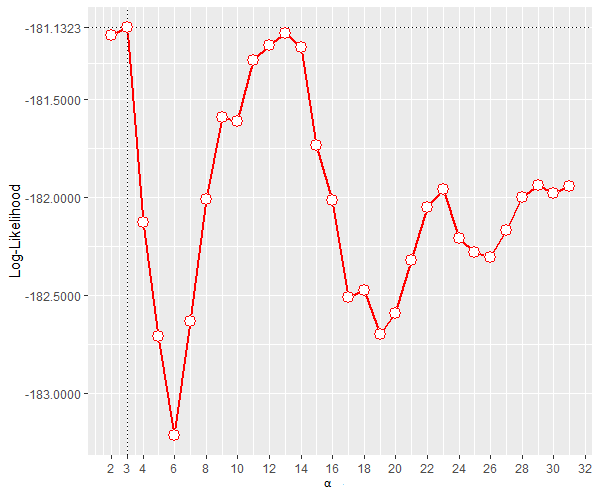
\includegraphics[width=0.49\textwidth]{AlphaBestPlot.png}
    \caption{Plot af likelihoodværdier mod $\alpha$. Parametrene i modellen er estimeret ud fra hver $\alpha$-værdi. Vi ser at den største likelihood opnås ved $\alpha=3$. }
    \label{fig:AlphaPlot}
\end{center}
\end{figure}
  og dermed beskrive en kamp ud fra 3 foregående runder. Det tager i gennemsnit 7 og 9 iterationer før konvergens for henholdsvis Rao-Kupper og den dynamiske model. Det skal bemærkes, at hver Newton-Rhapson iteration for den dynamiske model er 31 gange længere end for Rao-Kupper. 
  \begin{table}[ht]
\centering
\begin{adjustbox}{max width=\textwidth}
\begin{tabular}{|l|rrrr|rrrr|}
\hline
\multicolumn{1}{|l|}{} & \multicolumn{4}{l|}{Rao-Kupper} & \multicolumn{4}{l|}{Dynamisk Model} \\
\hline
Parameter & Estimat & SE &2.5\% &97.5\% & Estimat & SE &2.5\% &97.5\%\\
  \hline
    $\hat{\text{HjemmebaneFordel}}$ & -      & -     &      &            & 0.155 & 0.073  &0.012 & 0.298  \\
    $\hat{\text{SejrStreak}}$       & -      & -     &       &           & -0.152 & 0.122 &-0.392 & 0.088 \\
    $\hat{\text{FifaRating}}$       & -0.316 & 0.707 &-1.702 &1.069      & 0.392 & 0.152  &0.095 & 0.690 \\
    $\hat{\text{Hjørne}}$           & -0.437 & 0.980 &-2.359 &1.484      & 0.088 & 0.132  &-0.171 &0.347\\
    $\hat{\text{Offside}}$          &  0.126 & 0.312 &-0.485 &0.738      & -0.045 & 0.101 &-0.242 &0.152 \\
    $\hat{\text{MålScoret}}$        &  0.259 & 0.480 &-0.682 &1.200      & 0.112 & 0.138  &-0.159 &0.383\\
    $\hat{\text{MålLukketInd}}$     & -0.683 & 0.541 &-1.744 &0.378      & 0.104 & 0.117  &-0.125 & 0.333\\
    $\hat{\text{Tilskuere}}$        &  0.453 & 0.731 &-0.949&1.885       & 0.097 & 0.127 &-0.151 & 0.346\\
    $\hat{\text{Boldbesiddelse}}$   &  0.210 & 0.488 &-0.746 &1.166      & -0.042 & 0.136 &-0.309 & 0.225\\
    $\hat{\text{Skud}}$             &  0.160 & 0.540 &-0.899 &1.218      & 0.046 & 0.150 &-0.249 & 0.340\\
    $\hat{\text{SkudIndenfor}}$     & -0.395 & 0.770 &-1.904 &1.115      & -0.108 & 0.138 &-0.378 & 0.163\\
    $\hat{\text{Frispark}}$         & -0.214 & 0.418 &-1.033 &0.604      & -0.238 & 0.101 &-0.436 & -0.040\\
    $\hat{\theta}$                  & 1.667  & 0.121 &1.429  &1.904      & 1.663 & 0.123  & 1.422 & 1.904\\
   \hline
\end{tabular}
\end{adjustbox}
\caption{\label{tab:Parameterestimater}\textit{$\hat{\theta}$- og $\hat{\beta}$-koefficienter for sæson 2015 i superligaen, med Rao-Kupper til venstre, og den dynamiske model til højre}}
\end{table}
\\Vi ser i Tabel (\ref{tab:Parameterestimater}), at alle $\hat{\beta}$'erne i Rao-Kupper har store standardfejl og ikke er signifikante med et signifikansniveau på 5\%. $\hat{\theta}$ er signifikant, hvilket den er per definition, eftersom vi har uafgjorte kampe. I den dynamiske model, ser det en smule bedre ud, her er $\hat{HjemmebaneFordel}$, $\hat{FifaRating}$, $\hat{frispark}$ og $\hat{\theta}$ signifikante med et signifikansniveau på 5\%. For at sikre os at $\hat{\beta}$ i de to modeller samlet set er signifikante, udfører vi en kvotienttest med nulhypotesen:\\
$H_0$: $\beta_1=\beta_2=...=\beta_{12} = 0$.\\
Teststørrelserne bliver dermed for henholdsvis Rao-Kupper og den dynamiske model:\\
\begin{align*}
    -2\text{log}(Q_{RK})&=-2\Big{(}\ell_{RK} (\beta_{H_0}, \hat{\hat{\theta}})-\ell_{sta} (\hat{\beta},\hat{\theta})\Big{)}=-2(-211.233+190.644)=41.177\\
    -2\text{log}(Q_{dyn})&=-2\Big{(}\ell_{dyn} (\beta_{H_0},\hat{\hat{\theta}})-\ell_{dyn} (\hat{\beta},\hat{\theta})\Big{)}=-2(-198.033+181.078)=33.910
\end{align*}
Her er vores teststørrelse for $H_0$, ved store stikprøver, approksimativt $\chi^2_{10}$ fordelt for Rao-Kupper og $\chi^2_{12}$ fordelt for den dynamiske. De tilhørende $p$-værdier for Rao-Kupper og den dynamiske model er henholdsvis $0.00001$ og $0.0007$, hvorfor vi afviser nulhypotesen om, at $\beta$'erne er uden betydning for modellen. Vi konkluderer dermed, at der ikke er noget belæg for at fjerne $\beta$-parametrene helt fra modellen.
\\\\I Tabel \ref{tab:Styrkeestimater} sammenligner vi de to modellers rangering af holdene, og derudfra ser vi, at der er betydelig forskel på de to måder at anvende modellen på. Styrkerne for holdene er udregnet relativt til Hobro. Som forventet, kommer Rao-Kupper tættere på den faktiske rangering af holdene end den dynamiske model gør. Styrken for et hold i den dynamiske model, er beregnet som et gennemsnit af holdets styrke for alle runderne. De estimerede point, er udregnet ud fra de estimerede sandsynligheder tilhørende hver af kampene, hvor pointene tildeles ved: $3 \cdot p_{i \cdot ij}$ point til hold \textit{i}, $3\cdot p_{j \cdot ij}$ point til hold \textit{j} og $1\cdot p_{0 \cdot ij}$ point til begge hold. Bemærk at summen af de estimerede point ikke er lig summen af de observerede point, dette skyldes, at der er en forskel i antallet af estimerede uafgjorte kampe i forhold til de observerede uafgjorte kampe. Den sande sum af point er 552, hvor Rao-Kupper estimerer 551.947 og den dynamiske estimere 549.441. Det ses yderligere i Tabel \ref{tab:Styrkeestimater}, at for den dynamiske model, er holdenes rangering ud fra de gennemsnitlige styrker ikke den samme, som holdenes rangering ud fra point. Dette skyldes at der er en øvre grænse, for hvor mange point et hold kan få tildelt i en kamp, men der er ikke en øvre grænse for hvor stor styrken for et hold kan blive i en kamp. Denne øvre grænse vil altså kunne påvirke den gennemsnitlige styrke for et hold mere, end den vil kunne påvirke holdets antal point. 
\begin{table}[htb!]
\centering
\begin{adjustbox}{max width=\textwidth}
\begin{tabular}{|lr|rrrr|rrrr|}
\hline
\multicolumn{2}{|c|}{} & \multicolumn{4}{c|}{Rao-Kupper} & \multicolumn{4}{c|}{Dynamisk Model} \\
\hline
Hold & Point & Styrke & SE & Estimeret Point & Rangering & Styrke & SE & Estimeret Point & Rangering \\
  \hline
    FCK & 71 & 11.223 & 5.722 & 71.165 & 1  & 5.757 & 2.294 & 70.125 & 1 \\
    SJE & 62 & 7.048  & 3.463 & 61.029 & 2  & 1.717 & 0.437 & 43.156 & 8 \\
    FCM & 59 & 6.233  & 2.816 & 58.191 & 3  & 3.043 & 0.962 & 56.779 & 2 \\
    BIF & 54 & 5.075  & 2.432 & 53.367 & 4  & 2.281 & 0.698 & 49.854 & 4 \\
    AAB & 50 & 4.674  & 2.284 & 51.418 & 5  & 2.768 & 1.064 & 52.631 & 3 \\
    RFC & 47 & 4.032  & 1.901 & 47.923 & 6  & 1.999 & 0.516 & 47.115 & 6 \\
    OB  & 46 & 3.163  & 1.287 & 42.229 & 8  & 1.746 & 0.526 & 40.878 & 7 \\
    VFF & 40 & 2.880  & 1.335 & 40.068 & 9  & 1.173 & 0.290 & 33.485 & 10 \\
    FCN & 38 & 2.423  & 1.154 & 36.171 & 10 & 1.151 & 0.315 & 32.848 & 11 \\
    AGF & 37 & 3.173  & 1.500 & 42.299 & 7  & 1.662 & 0.407 & 40.474 & 9 \\
    EFB & 30 & 1.744  & 0.071 & 29.161 & 11 & 2.012 & 0.442 & 47.995 & 5 \\
    HOB & 18 & 1.000  & 0.000 & 18.926 & 12 & 1.000 & 0.000 & 34.102 & 12 \\
   \hline   
\end{tabular} 
\end{adjustbox}
\caption{\label{tab:Styrkeestimater}\textit{Rangering af holdene i forhold til deres styrker, samt deres forventede antal point ved slutningen af sæsonen. Styrkerne er udregnet relativt til Hobro}}
\end{table}
\\Det viser sig, at der er markant flere hjemmebanesejre end udebanesejre. Figur \ref{fig:boxplot} viser boxplot af estimerede sandssynligheder mod observerede udfald. Vi ser, at den dynamiske model \ref{fig:boxplotD} estimerer fordelingen af hjemmebanesejre, udebanesejre og uafgjorte kampe bedre i forhold til de observerede udfald af kampene, end Rao-Kupper \ref{fig:boxplotS}. De stiblede linjer (rød, blå, grøn) viser de observerede middelværdier for hhv (hjemmesejr, udesejr, uafgjort).
\begin{table}[htb!]
\centering
\begin{adjustbox}{max width=\textwidth}
\begin{tabular}{|l|ccc|}
\hline 
 & Hjemmmesejr & Udesejr & Uafgjort \\
 \hline
Observeret & 0.460 & 0.328 & 0.212\\
Rao Kupper & 0.396 & 0.391 & 0.213\\
Dynamisk Rao Kupper & 0.463 & 0.322 & 0.215\\
   \hline   
\end{tabular} 
\end{adjustbox}
\caption{\label{tab:HjemmeUdeProcenter}\textit{Procentvise observerede og estimerede udfald for Rao Kupper modellen samt den Dynamiske Rao Kupper Model}}
\end{table}\\
At den dynamiske model estimerer den observerede fordeling af (hjemmesejr, udesejr, uafgjort) bedre, skyldes at den dynamiske model tager højde for hjemmebanefordelen. At Rao-Kupper estimaterne for hjemmesejrer og udesejrer ikke er ens, skyldes at alle hold i sæsonen ikke spiller lige mange hjemme og udebanekampe. Det medfører at modellen vil estimere flere hjemmesejrer, hvis det er de hold med de største styrker, som spiller en ekstra hjemmebane kamp. 
\begin{figure}[h!]
  \centering
  \begin{subfigure}[b]{0.475\linewidth}
    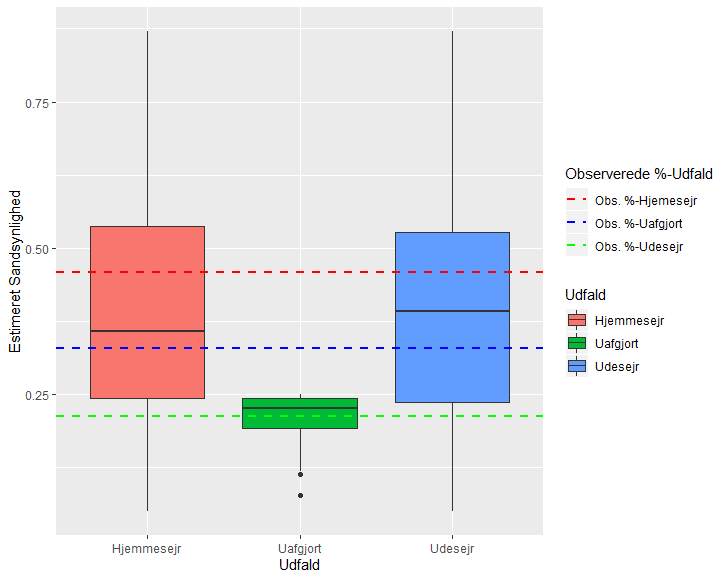
\includegraphics[width=\linewidth]{EstSSHStatisk.png}
    \caption{Rao Kupper}
    \label{fig:boxplotS}
  \end{subfigure}
  \begin{subfigure}[b]{0.475\linewidth}
    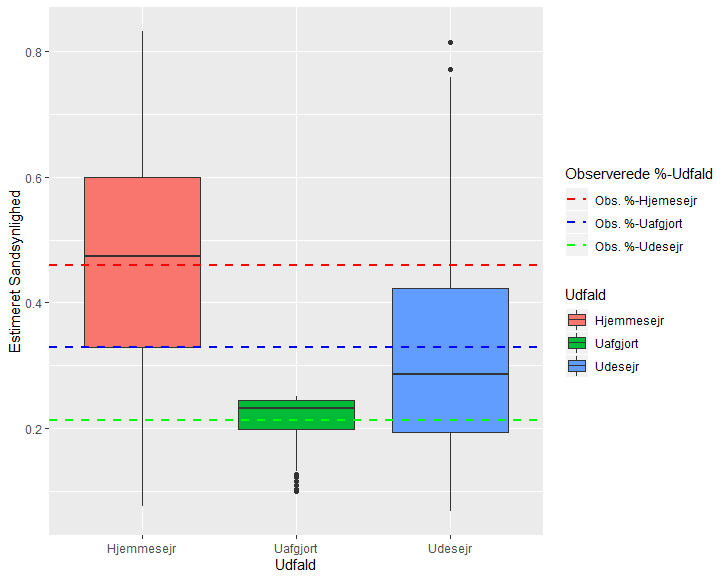
\includegraphics[width=\linewidth]{EstSSHDyn.png}
    \caption{Dynamisk}
    \label{fig:boxplotD}
  \end{subfigure}
  \caption{\textit{Boksplot af estimerede sandsynligheder mod observerede udfald. De røde, blå og grønne boksplot viser fordelingerne af hhv. estimerede hjemmesejrer, udesejrer og uafgjorte kampe. De stiplede linjer viser de emperiske middelværdier for de observerede udfald.}}
  \label{fig:boxplot}
\end{figure}

For at se nærmere på de estimerede sandsynligheder, kigger vi på deres respons-residualer mod fittede værdier for de tre udfald; dette ses i Figur \ref{fig:residualplot}. Den sorte linje viser middelværdien af residualerne, og den røde linje er en kerneudglatning. Båndbredderne er valgt ved at tage udgangspunkt i \textit{R}-funktionen {\fontfamily{qcr}\selectfont dpill}, og efterfølgende rettet til. Vi ser, at middelværdierne for den dynamiske model er tættere på 0 end de er for Rao-Kupper. Rao-Kupper har en middelværdi over 0 for hjemmesejr og under 0 for udesejr. Dette er en forventelig følge, da Rao-Kupper generelt vil overestimere sandsynligheden for udesejr og underestimere sandsynligheden for hjemmesejr. Idet den ikke inkorporerer nogen hjemmebaneparameter. Der ser ikke ud til at danne sig noget klart mønster for de fittede værdier, dog er der noget støj ved halerne. Residualerne tilhørende de uafgjorte kampe er meget ens for de to modeller, hvilket også måtte forventes, da $\theta$ er meget ens for dem. Der er dog en lidt større spredning for uafgjort i de fittede værdier for den dynamiske model, hvilket skyldes forskellen i $\beta$'erne, og især implementeringen af hjemmebanefordelen. Det er generelt svært at sige noget konkret om disse residualer, eftersom vi har så få observationer i hver kategori. Derfor vælger vi heller ikke at fjerne nogle af de outliers der befinder sig i halerne.
\begin{figure}[h!]
  \centering
  \begin{subfigure}[b]{0.425\linewidth}
    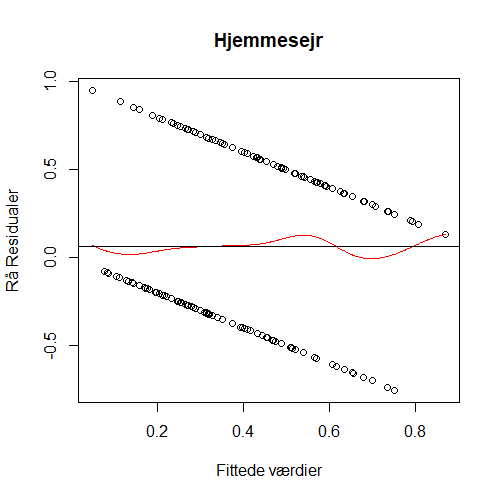
\includegraphics[width=\linewidth]{ResSHS.png}
    \caption{Rao-Kupper med båndbredde 0.08}
    \label{fig:ResSHS}
  \end{subfigure}
  \begin{subfigure}[b]{0.425\linewidth}
    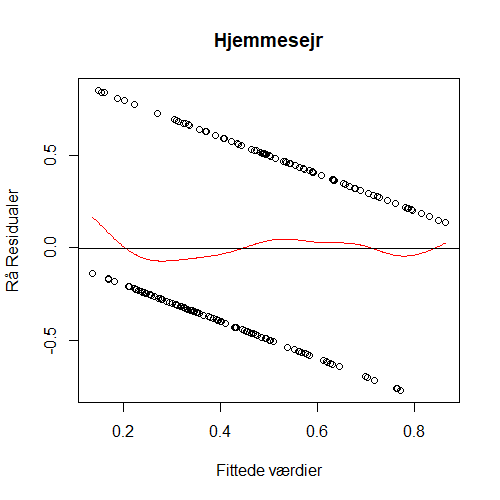
\includegraphics[width=\linewidth]{ResDHS.png}
    \caption{Dynamisk med båndbredde 0.05}
    \label{fig:ResDHS}
  \end{subfigure}
  \begin{subfigure}[b]{0.425\linewidth}
    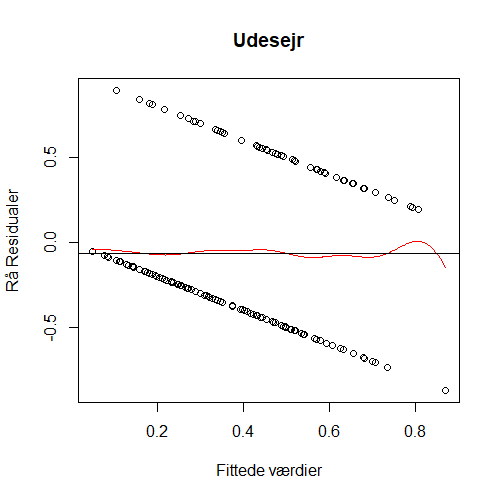
\includegraphics[width=\linewidth]{ResSUS.png}
    \caption{Rao-Kupper med båndbredde 0.075}
    \label{fig:ResSUS}
  \end{subfigure}
  \begin{subfigure}[b]{0.425\linewidth}
    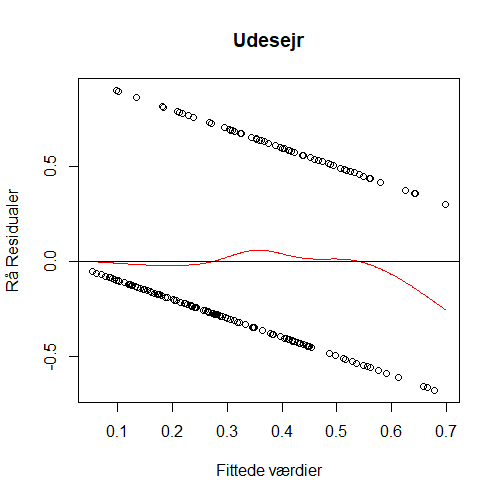
\includegraphics[width=\linewidth]{ResDUS.png}
    \caption{Dynamisk med båndbredde 0.075}
    \label{fig:ResDUS}
  \end{subfigure}
  \begin{subfigure}[b]{0.425\linewidth}
    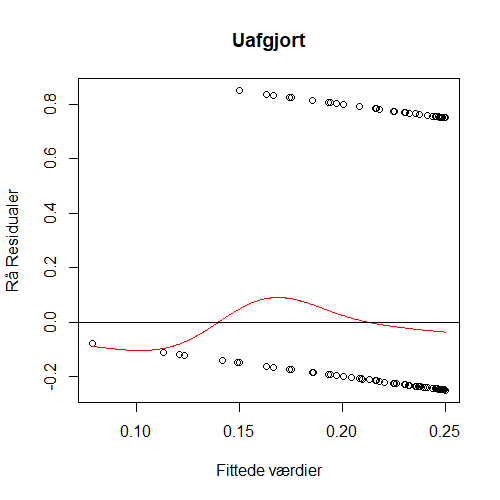
\includegraphics[width=\linewidth]{ResSU.png}
    \caption{Rao-kupper med båndbredde 0.02}
    \label{fig:ResSU}
  \end{subfigure}
  \begin{subfigure}[b]{0.425\linewidth}
    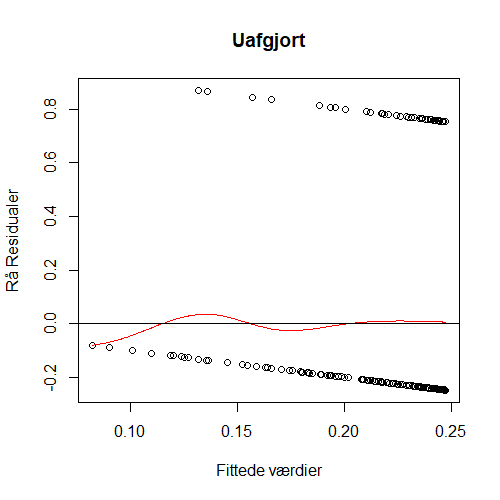
\includegraphics[width=\linewidth]{ResDU.png}
    \caption{Dynamisk med båndbredde 0.02}
    \label{fig:ResDU}
  \end{subfigure}
  \caption{\textit{Residualer mod fittede værdier. Den røde linje viser en Nadaraya-Watson udglatning med normal kerne. De tilhørende båndbredder er valgt med udgangspunkt i R-funktionen dpill, og efterfølgende tilpasset.}}
  \label{fig:residualplot}
\end{figure}
\clearpage
\section{Lasso}
I dette afsnit viser vi, hvordan vi ved brug af lassostraf ($l_1$ norm straf) udvælger de mest beskrivende parametre, og sætter deres koefficienter derefter. Formålet er, at forbedre vores models prædiktionsevne ved at mindske modellens forventede prædiktionsfejl, eller med andre ord maksimalisere likelihooden på noget fremmed data. Til sidst viser vi, hvordan vi implementerer lasso i vores algoritmer med udgangspunkt i den dynamiske model.\\\\
\subsection{Tabsfunktioner}
Når vi beregner prædiktionsfejl, kræver det, at vi noget har testdata som vi ikke har fitted vores model ud fra. Det vil sige, at vi fitter vores model på et træningsdatasæt, for derefter at teste den på et andet testdatasæt. Givet et datasæt med observationerne $\{1,...,N\}$, kalder vi træningsdatasættet for $n$ og testdatasættet for $q$; så $\{1,...,N\}\rightarrow\{1_n,...,N_n,1_q,...,N_q\}$ er en indeksering af observationerne i forhold til hvorvidt de bliver anvendt til at fitte vores model eller teste den. En metode til at måle modellens prædiktionsfejl på, er \textit{mean squarred prediction error} (MSPE). I MSPE udregnes den kvadrede prædiktionsfejl for hver af sandsynlighederne ($p_{i\cdot ij}, p_{j\cdot ij}, p_{0\cdot ij}$) individuelt, og MSPE for en kamp mellem hold $i$ og hold $j$ bliver summen af de kvadrede prædiktionsfejl for hver af de tre estimerede sandsynligheder. MSPE for at hold $i$ vinder over hold $j$ bliver:
\begin{align*}
\text{MSPE}\big{(}\hat{p}_{i\cdot ij}\big{)}=&E\Big{[}\big{(}y_{i\cdot ij}-\hat{p}_{i\cdot ij}\big{)}^2\Big{]}\\
=&E\Big{[}\big{(}\hat{p}_{i\cdot ij}-E\big{[}\hat{p}_{i\cdot ij}\big{]}+E\big{[}\hat{p}_{i\cdot ij}\big{]}-y_{i\cdot ij}\big{)}^2\Big{]}\\
=&E\Big{[}\big{(}\hat{p}_{i\cdot ij}-E\big{[}\hat{p}_{i\cdot ij}\big{]}\big{)}^2+2\big{(}\hat{p}_{i\cdot ij}-E\big{[}\hat{p}_{i\cdot ij}\big{]}\big{)}\big{(}E\big{[}\hat{p}_{i\cdot ij}\big{]}-y_{i\cdot ij}\big{)}\\
&+\big{(} E\big{[}\hat{p}_{i\cdot ij}\big{]}-y_{i\cdot ij}\big{)}^2\Big{]}\\
=&E\Big{[}\big{(}\hat{p}_{i\cdot ij}-E\big{[}\hat{p}_{i\cdot ij}\big{]}\big{)}^2\Big{]}
+2\underbrace{\big{(}E\big{[}\hat{p}_{i\cdot ij}\big{]}-E\big{[}\hat{p}_{i\cdot ij}\big{]}\big{)}}_{0}\big{(}E\big{[}\hat{p}_{i\cdot ij}\big{]}-y_{i\cdot ij}\big{)}\\
&+\big{(} E\big{[}\hat{p}_{i\cdot ij}\big{]}-y_{i\cdot ij}\big{)}^2\\
=&E\Big{[}\big{(}\hat{p}_{i\cdot ij}-E\big{[}\hat{p}_{i\cdot ij}\big{]}\big{)}^2\Big{]}+\Big{(} E\big{[}\hat{p}_{i\cdot ij}\big{]}-y_{i\cdot ij}\Big{)}^2\\
=&Var\Big{(}\hat{p}_{i\cdot ij}\Big{)}+\text{Bias}^2\Big{(}\hat{p}_{i\cdot ij}\Big{)},\\
\intertext{Vi ser at prædiktionsfejlen er en funktion af den kvadrerede bias af vores estimat og variansen af vores estimat. Det vil sige, at vi minimaliserer vores prædiktionsfejl ved at minimalisere bias og varians. MSPE for alle de estimerede udfald af kampene mellem hold $i$ og hold $j$ bliver:}
\text{MSPE}\big{(}\hat{p}_{ij}\big{)}&=\text{MSPE}\big{(}\hat{p}_{i\cdot ij}\big{)}+\text{MSPE}\big{(}\hat{p}_{j\cdot ij}\big{)}+\text{MSPE}\big{(}\hat{p}_{0\cdot ij}\big{)},\\
\intertext{MSPE tabsfunktionen med træningsdatasæt $n$ og testdatasæt $q$ er:}
\mathcal{T}_{\text{MSPE}}\big{(}\hat{\beta}_{-q},\hat{\theta}_{-q}|x,y_{ij},n,q\big{)}&=\frac{1}{N_q}\sum_{t\in q}\sum_{i<j}\Big{[}\big{(}y_{i\cdot ij}(t)-\hat{p}_{i\cdot ij}(t)\big{)}^2+\big{(}y_{j\cdot ij}(t)-\hat{p}_{j\cdot ij}(t)\big{)}^2+\big{(}y_{0\cdot ij}(t)-\hat{p}_{0\cdot ij}(t)\big{)}^2\Big{]},
\end{align*}
hvor $-q$ i $\hat{\beta}_{-q}, \hat{\theta}_{-q}$ viser at parametrene er estimeret uden observationer fra testdatasættet $q$, og $N_q$ er antal observationer i testdatasættet.\newline\newline
En anden hyppigt anvendt tabsfunktion i klassificeringsproblemer er \textit{logistic loss}\cite{LineSearch} (log loss) også kendt som \textit{cross entropy loss}. I log loss er den forventede prædiktionsfejl beregnet i forhold til hvor langt væk den estimerede sandsynlighed for det observerede udfald er fra 1; log loss prædiktionsfejlen i en kamp mellem hold $i$ og hold $j$ i runde $t$ bliver:
\begin{align*}
    \mathcal{T}_{\log} \big{(}p_{ij}(t)\big{)}
    &=-\Big{(}y_{i\cdot ij}(t)\log\big{(}\hat{p}_{i\cdot ij}(t)\big{)}+y_{j\cdot ij}(t)\log\big{(}\hat{p}_{j\cdot ij}(t)\big{)}
    +y_{0\cdot ij}(t)\log\big{(}\hat{p}_{0\cdot ij}(t)\big{)}\Big{)},\\
\intertext{og log tabsfunktionen for hele testsættet bliver:}
\mathcal{T}_{\log}\big{(}\hat{\beta}_{-q},\hat{\theta}_{-q}|x,y_{ij},n,q\big{)}
&=-\frac{1}{N_q}\sum_{t\in q}\sum_{i<j}\Big{(}y_{i\cdot ij}(t)\log\big{(}\hat{p}_{i\cdot ij}(t)\big{)}
+y_{j\cdot ij}(t)\log\big{(}\hat{p}_{j\cdot ij}(t)\big{)}
+y_{0\cdot ij}(t)\log\big{(}\hat{p}_{0\cdot ij}(t)\big{)}\Big{)}.\\
\intertext{Ved at sammenligne med likelihood funktionen ser vi, at minimalisere log tabsfunktionen er ækvivalent med at minimalisere den negative log likelihood (maksimalisere log likelihooden) over testsættet:}
-\ell\big{(}\hat{\beta}_{-q},\hat{\theta}_{-q}\big{)}
&=-\log\prod_{t\in q}\prod_{i<j}\hat{p}_{i\cdot ij}(t)^{y_{i\cdot ij}(t)}\hat{p}_{j\cdot ij}(t)^{y_{j\cdot ij}(t)}\hat{p}_{0\cdot ij}(t)^{y_{0\cdot ij}(t)}\\
&=-\sum_{t\in q}\sum_{i<j}\Big{(}y_{i\cdot ij}(t)\log\big{(}\hat{p}_{i\cdot ij}(t)\big{)}+y_{j\cdot ij}(t)\log\big{(}\hat{p}_{j\cdot ij}(t)\big{)}+y_{0\cdot ij}(t)\log\big{(}\hat{p}_{0\cdot ij}(t)\big{)}\Big{)}.
\end{align*}
\subsection{Lasso-metoden}
Indtil videre har vi anvendt alle vores forklarende variable, til at beskrive de forskellige fodboldholds styrker. Der er altså en risiko for, at vi overfitter vores model med overflødige variable, som enten beskriver; den samme varians, beskriver den dårligt, eller slet ikke beskriver den. I dette afsnit vil vi tage udgangspunkt i det velkendte ordsprog \textit{"less is more"}, og forsøge at indskærpe modellen, så de bedste variable vægtes mest og de dårligere enten vægtes mindre eller fjernes helt. Robert Tibshirani (1996)\cite{RobertTibshirani} foreslår en metode kaldet lasso \textit{(least absolute shrinkage and selection operator)} til at identificere, hvor godt de forskellige parametre beskriver udfaldene og justerer deres koefficienter derefter. Lasso-optimeringsproblemet tager som tidligere udgangspunkt i at maksimalisere likelihooden, men nu under en bibetingelse:
\begin{align*}
&\max_{\beta,\,\theta} \Big{\{}\ell(\beta,\theta)\Big{\}} \\
&\text{u.b.b. }\sum_{i=1}^k|\beta_i|\leq s,
\end{align*}
hvor bibetingelsen straffer i forhold til de normerede $\beta$-koefficienter. $s$, som beskriver den størst mulige sum af $\beta$-koefficienterne, er en brugervalgt strafparameter. 
Vi omskriver lasso-problemet på \textit{Lagrange-form}, da vi senere hen benytter dets praktiske implementerbarhed:
\begin{align*}
\max_{\beta,\,\theta} \Big{\{}\ell(\beta,\theta)-\lambda\sum_{i=1}^k|\beta_i|\Big{\}}=\min_{\beta,\,\theta} \Big{\{}-\ell(\beta,\theta)+\lambda\sum_{i=1}^k|\beta_i|\Big{\}},\text{ hvor }\beta
\end{align*}
hvor $\lambda\geq0$ er en strafparameter tilsvarende $s$, og beskriver hvor objektfunktionen skal straffes i forhold de normerede $\beta$-koefficienter. $\lambda$ og $s$ har et inverst forhold, så når $\lambda$ er høj, er $s$ lav. Sammenhængen mellem $s$ og $\lambda$ er vist for en lineær model med ortogonal designmatrice i slutningen næste underafsnit (4.3).


\subsection{Lineær Model med Ortogonal Designmatrice Eksempel}
For at forklare effekten af lasso på parametrene, vil vi tage udgangspunkt i en lineær model med ortogonal designmatrice, fordi vi i det tilfælde kan skrive resultatet ned eksplicit. Når X er ortogonal er $X^T=X^{-1}$, så \textit{least squares} løsningen bliver:
\begin{align*}
\hat{\beta}=\big{(}X^TX\big{)}^{-1}X^Ty=X^Ty.
\end{align*}
Lasso-problemet for en lineær model bliver:
\begin{align*}
&\min_\beta \Big{\{}\big{(}y-X\beta\big{)}^T\big{(}y-X\beta\big{)}+\lambda\sum_{i=1}^k|\beta_i|\Big{\}}=\min_\beta \Big{\{}y^Ty+X^TX\beta^T\beta-2y^TX\beta+\lambda\sum_{i=1}^k|\beta_i|\Big{\}},\\
\intertext{da $y^Ty$ er uafhængig af $\beta$, $X^TX=1$ og $\hat{\beta}=X^Ty$ omskriver vi problemet til:}
&\min_\beta \Big{\{}2\beta^2-\hat{\beta}\beta+\lambda\sum_{i=1}^k|\beta_i|\Big{\}}=\min_\beta \Big{\{}\sum_{i=1}^k\Big{(}2\beta_i^2-\hat{\beta_i}\beta_i+\lambda |\beta_i|\Big{)}\Big{\}}.\\
\intertext{Objektfunktion er nu en sum af k identiske problemer, som vi løser hver for sig. Vi tager udgangspunkt i det i'te problem, og får objektfunktionen:}
&f(\beta_i)=-2\hat{\beta}_i\beta_i+\beta_i^2+\lambda|\beta|.\\
\intertext{Eftersom vi ønsker at minimere objektfunktionen må det gælde, at $\hat{\beta}_i>0\rightarrow\beta_i\geq0$, for ellers ville objektfunktionen kunne mindskes ved at skifte fortegnet for $\beta_i$, og ligeledes må det gælde, at $\hat{\beta}_i<0\rightarrow\beta_i\leq0$ Ved at differentier og sætte lig 0 fås den afledte:}
&f'(\beta_i)=-2\sgn\big{(}\hat{\beta_i}\big{)}\hat{\beta_i}+2\beta_i+\lambda. \\
\intertext{Ved at isolere $\beta_i$ og gange begge sider med fortegnet for $\beta_i$ (fortegnet for $\hat{\beta_i}$), for at sikre positivt fortegn på venstre siden, fås:}
&\beta_i=\sgn\big{(}\hat{\beta_i}\big{)}\Big{(}\sgn\big{(}\hat{\beta_i}\big{)}\hat{\beta_i}-\frac{1}{2}\lambda\Big{)}=\sgn\big{(}\hat{\beta_i}\big{)}\big{(}|\hat{\beta_i}|-\frac{1}{2}\lambda\big{)},\\
\intertext{hvis $\hat{\beta}_i<0$ kræves, at $\sgn\big{(}\hat{\beta_i}\big{)}\big{(}|\hat{\beta_i}|-\frac{1}{2}\lambda\big{)}\leq0$ og ligeledes kræver $\hat{\beta}_i>0$, at $\sgn\big{(}\hat{\beta_i}\big{)}\big{(}|\hat{\beta_i}|-\frac{1}{2}\lambda\big{)}\geq0$, hvilket løses ved at sætte $\big{(}|\hat{\beta_i}|-\frac{1}{2}\lambda\big{)}$ lig nul, hvis ledet er negativt:}
&\hat{\beta}_i^{\text{lasso}}=\sgn\big{(}\hat{\beta_i}\big{)}\big{(}|\hat{\beta_i}|-\frac{1}{2}\lambda\big{)}^{+},\\
\end{align*}
\begin{align}
\intertext{så}
 &\hat{\beta}^{\text{lasso}}=\sgn\big{(}\hat{\beta}\big{)}\big{(}|\hat{\beta}|-\frac{1}{2}\lambda\big{)}^{+}\label{lig:LassoLøsning}
\end{align}
Vi ser tydeligt, at når $\lambda$ stiger, går $\hat{\beta}_i^{\text{lasso}}$ mod 0, samt at $\lambda\geq2|\hat{\beta}_i|\rightarrow \hat{\beta}_i^{\text{lasso}}=0$. Det vil sige, at i forbindelse med at $\lambda$ stiger vil lasso-estimaterne gå mod 0, samt at når $\lambda$ bliver tilpas stor vil en eller flere koefficienter sættes lig 0, hvilket betyder at lasso løbende træffer et valg af underum. Idéen er nu, at når $|\beta|$-koefficienterne mindskes, mindskes variansen af de estimerede sandsynligheder, hvilket medfører at modellens prædiktionsfejl mindskes. Dette sker dog på bekostning af, at når $|\beta|$-koefficienterne mindskes, medfører det også at den kvadrerede bias stiger, hvilket øger modellens forventede fejl. Variansen falder, da sandsynlighederne bliver mindre påvirket af deres kovariater. Den kvadrerede bias stiger, da lasso trækker estimaterne mod 0 og væk fra de centrale løsninger. Ved justering af $\lambda$ bliver modellens forventede prædiktionsfejl altså trukket i hver sin retning på grund af ændringer i bias og varians. Dette forhold mellem bias og varians kaldes \textit{The Bias-Variance Decomposition} \cite{ESL}. Humlen er så, at finde den $\lambda$ der minimaliserer de forventede prædiktionsfejl.\par
Vi ønsker at vise forholdet mellem $\lambda$ og $s$, og vil gøre det med udgangspunkt i den lineære model med ortogonal designmatrice, hvor vi kender lasso-løsningen: Lad $f:\rm I\!R^k \rightarrow \rm I\!R$ være en konveks tabsfunktion, så vil for et hvilket som helst vektor-par $(\beta, \hat{\beta})$ i $f$'s mængde og for en $b\in [0,1]$ gælde, at
\begin{align*}
    f(b\beta+(1-b)\hat{\beta})&\leq bf(\beta)+(1-b)f(\hat{\beta}),
\intertext{hvilket betyder, at en linje mellem to $f(\beta)$ og $f(\hat{\beta})$ altid vil ligge på eller over grafen for f. Det medfører, at hvis en konveks funktion har et lokalt minimumspunkt er det også et globalt minimumspunkt. $\hat{\beta}$ er globalt minimumspunkt, hvis}
    bf(\beta)+(1-b)f(\hat{\beta})&\leq bf(\beta)+(1-b)f(\beta)=f(\beta), 
\intertext{for alle $\beta$ i $f$'s mængde. Det betyder, at $bf(\beta)+(1-b)f(\hat{\beta})$ er bedre end $f(\beta)$ medmindre $f(\beta)=f(\hat{\beta})$ eller $b=1 \iff f(\beta)=f(\beta)$. Lad nu bibetingelsen $|\beta| \leq s$ være aktiv, så $s\leq|\hat{\beta}|$ og lad $|\Tilde{\beta}|<s$. Så vil det gælde, at}
&|\Tilde{\beta}|\leq b|\Tilde{\beta}|+(1-b)|\hat{\beta}|, 
\intertext{hvor}
&b|\Tilde{\beta}|+(1-b)|\hat{\beta}|\leq s
\intertext{hvis blot b er lille nok. Dermed findes der et bedre punkt end $\Tilde{\beta}$ med 1-norm mindre end $s$. Dermed kan $\Tilde{\beta}$ ikke være minimumspunkt for $f$ u.b.b $\beta\leq s$. Derfor må minimumspunktet $\hat{\beta}$ for konvex funktion $f$ u.b.b $|\beta|\leq s$ have 1-norm lig $s$. Figur \ref{fig:lasso1dim} viser et eksempel på minimaliserings problemet af en konvekse funktion $f=\beta^2-5\beta$, u.b.b $|\beta|\leq s=1$, hvor $\beta \in \rm I\!R$.}
\end{align*}
Nu kan vi med udgangspunkt i $\hat{\beta}^{\text{lasso}}$-løsningen fra ligning (\ref{lig:LassoLøsning}), opstille $s$ som funktion af $\lambda$ når $0 < s < \sum_i^k\hat{\beta}_i$ (s er aktiv og større end nul):
 \begin{align*}
s&=\sum_i^k\Big{(}|\hat{\beta}_i^{\text{lasso}}|\big{)}=\sum_i^k\big{(}|\hat{\beta}_i|-\frac{1}{2}\lambda\big{)}^{+}
\intertext{hvorfra vi tydeligt ser, at der er en én til én korrespondance mellem $s$ og $\lambda$, hvor s er lav når $\lambda$ er høj. Vi ser, at hvis $s=\frac{1}{\delta}\sum_i^k\|\beta_i|$ vil koefficienterne gennemsnitligt mindskes til $\frac{1}{\delta}$ af hvad de var før,samt $s\geq \hat{\beta}\iff \lambda=0$, hvor $\hat{\beta}^{\text{lasso}}=\hat{\beta}$.}
\end{align*}
Figur \ref{fig:lasso2dim} er hentet fra Elements of Statistical Learning \cite{ESL}, og viser en todimensionel løsning til et lasso-optimeringsproblem. Den blå firkant illustrer L1-norm bibetingelsen $|\beta_1| + |\beta_2| \leq s$. De røde elipser viser niveaukurver for tabsfunktionen, og løsningen ligger på randen af s og vil være den elipse der kommer tættest på $\hat{\beta}$(least square løsningen). Hvis løsningen er en hjørneløsningen vil en af parametrene være 0, som vist på figuren (hvor $\beta_1=0$). 
\begin{figure}[h!]
  \centering
    \begin{subfigure}[b]{0.48\linewidth}
    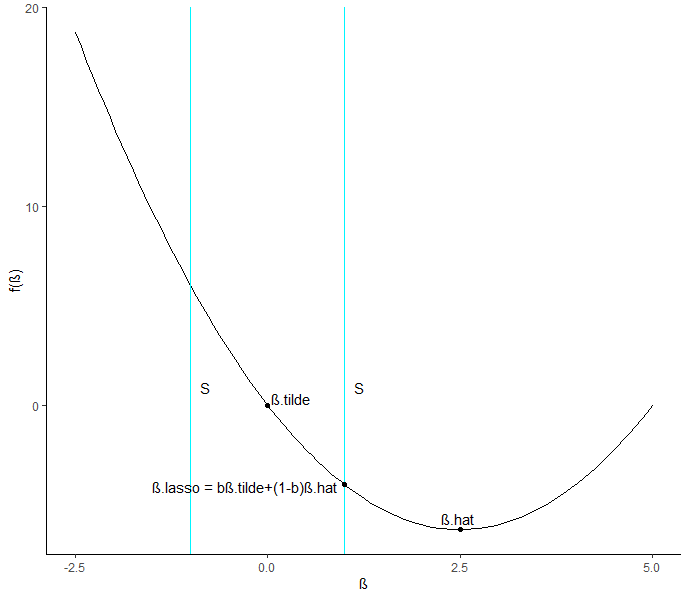
\includegraphics[width=\textwidth]{LAMBDABETA.png}
    \caption{}
  \label{fig:lasso1dim}
  \end{subfigure}
  \begin{subfigure}[b]{0.48\linewidth}
    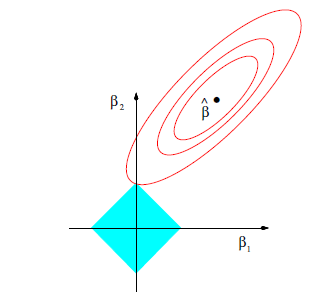
\includegraphics[width=\textwidth]{Lasso-ESL.PNG}
    \caption{}
    \label{fig:lasso2dim}
  \end{subfigure}
  \caption{\textit{Venstre figur (a) illustrerer lasso-løsningen med én parameter, og viser minimaliseringsproblemet af tabsfunktionen $f=\beta^2-5\beta$ under L1-norm bibetingelsen $s$. De lodrette blå streger illustrerer bibetingelsen $|\beta|\leq s=1$. Højre Figur (b) er en illustration af lassoløsningen med to parametre. Den blå firkant illustrerer L1-norm bibetingelsen $|\beta_1| + |\beta_2| \leq  s$ og de røde elipser er niveaukurver af objektfunktionen. Højre figur er hentet fra Elements of Statistical Learning \cite{ESL}}.}
\label{fig:lassofigure}\end{figure}
\subsection{Standardfejl}
Standardfejl på parametre estimeret ved brug af lassostraf er er stadig et diskuteret emne. Da lasso estimaterne hverken er lineære eller differentiable er det svært at beregne præcise standardfejl. En løsning til dette problem er, at approksimere lasso-straffen med en differentiabel funktion. Ved en differentiabel approksimation kan kovariansmatricen approksimeres som sædvanlig, ved den inverse observation, og standardfejlene som kvadratroden af dennes diagonal. Der er dog stadig det problem, at de estimerede standardfejl tilhørende paramtrene som er blevet fravalgt (straffet ud af modellen) vil være 0, hvilket er misvisende.

\subsection{Implementering af lasso}
Fremgangsmåden i implementeringen af lasso er den samme for vores to versioner af Rao-Kupper modellen. Derfor vælger vi som nævnt, at tage udgangspunkt i den dynamiske model, når vi viser, hvordan vi implementerer lasso. \par
Ændringerne i de estimerede sandssynligheder ved implementering af lasso, sker i det $\hat{\beta}^{\text{lasso}}$-koefficienterne bliver funktioner af $\lambda$. Som vist for en lineær model med ortogonal designmatrice. I den dynamiske Rao-Kupper model med lasso-straf opskriver vi den forventede sandsynlighed for at hold $i$ vinder over hold $j$ som:
\begin{align}
    \hat{p}^{\text{lasso}}_{i\cdot ij}(t)
    &=\frac{\hat{\pi}_i\big{(}x_i(t,\alpha),\hat{\beta}(\lambda)\big{)}}{\hat{\pi}_i\big{(}x_i(t,\alpha),\hat{\beta}(\lambda)\big{)}+\hat{\theta}\hat{\pi}_j\big{(}x_j(t,\alpha),\hat{\beta}(\lambda)\big{)}}\nonumber\\
    &=\frac{1}{1+e^{-\big{(}x_i^T(t,\alpha)\hat{\beta}(\lambda)-x_j^T(t,\alpha)\hat{\beta}(\lambda)-\eta\big{)}}}.
    \label{func:pdynlasso}
\end{align}
Da Newton-Rhapson algoritmen kræver, at funktionen der ønskes maksimaliseret er to gange differentiabel, og strafledet $\lambda |\beta|$ kun er én gang differentiabel med hensyn til $\beta$, approksimerer vi strafledet med den glatte funktion $\lambda(\sqrt{\beta^2+C^2})\approx\lambda |\beta|$ når $C\rightarrow 0$. Bemærk at vi i resten af projektet refererer til dette strafled som lasso, på trods af at det er en approksimation. Maksimaliseringsproblemet til estimering og udvælgelse af lassoparametrene bliver:
\begin{align*}
\max_{\beta,\,\theta} &\Big{\{}\ell\Big{(}\beta,\theta\Big{|}x(t,\alpha),y_{ij}(t),r_{ij}(t)\Big{)}-\lambda \Big{(}\sqrt{\beta^2+C^2}\Big{)}\Big{\}}\\
=\max_{\beta,\,\theta} 
&\Big{\{}\sum_{t}\sum_{i<j}\Big{[}y_{i\cdot ij}(t)\log\Big{(}\frac{\pi_i}{\pi_i+\theta\pi_j}\Big{)}
+ y_{j\cdot ij}(t)\log\Big{(}\frac{\pi_j}{\pi_j+\theta\pi_i}\Big{)}\\
&+ \big{(}r_{ij}(t)-y_{i\cdot ij}(t)-y_{j\cdot ij}(t)\big{)} \log\Big{(}\frac{(\theta^2-1)\pi_i \pi_j}{(\pi_i+\theta\pi_j)(\pi_j+\theta\pi_i)}\Big{)}\Big{]}-\lambda \Big{(}\sqrt{\beta^2+C^2}\Big{)}\Big{\}},
\end{align*}
hvor $\pi_i=e^{\big{(}x_i^T(t,\alpha),\beta(\lambda)\big{)}}$. For at gøre konvergeringen hurtigere initialiseres problemet med maksimum likelihood estimaterne $\hat{\beta}$ og $\hat{\theta}$. Udvælgelsen af parametrene sker ved baglæns elimination, hvor vi initialisere med samtlige parametre og efterfølgende fjerner dem hvis de bliver 0. Idet vi løser problemet numerisk, er det nødvendigt at have en grænseværdi for, hvornår vi anser en parameter tæt nok på 0 til at være 0. Efter \textit{trial and error}, synes vi, at en nedre grænseværdi på $10^{-5}$ for parametrene virker fornuftig, og giver en fin spredning af fravælgelsen; så hvis $\beta_k<10^{-5}$ eller fortegnet for $\beta_k$ ændres ved en Newton-Rhapson iteration, sættes $\beta_k=0$. Hvis grænsen sættes meget strengere, vil parametrene kunne sættes markant under vores Newton-Rhapson konvergerings tolerence for samlet ændring i parametrene på $10^{-6}$, og derfor ikke blive fjernet. Hvis grænsen sættes meget mildere, vil de fleste parametre blive fjernet allerede ved meget lave $\lambda$ værdier, og det vil derfor være svært at skelne mellem hvor godt de forskellige parametre beskriver styrkerne. Figur \ref{fig:DBetaLasso} viser $\hat{\beta}^{\text{lasso}}$-koefficienterne mod $\lambda$ i den dynamiske model, og den tilhørende algoritme til estimering og udvælgelse af parametrene er skrevet som pseudokode i \textit{Algorithm 3}.\\
\begin{algorithm}[H]
\SetAlgoLined
\KwResult{$\max_{\beta,\,\theta} \Big{\{}\ell\Big{(}\beta,\theta|x,y_{ij}(t),r_{ij}(t),\lambda\Big{)}\Big{\}}$}
 Initialisér $v_0 = \begin{bmatrix}
           \beta \\
           \theta
         \end{bmatrix} =\begin{bmatrix}
           \beta_0 \\
           \theta_0
         \end{bmatrix}\;$\\
 \For{($c = 0,1,..., $ indtil konvergens)}{
  \For{$(t = 3,...,SlutRunde)$}{
        \eIf{($\alpha\geq t$)}{$\alpha_1 = t-1\;$}{$\alpha_1 = \alpha\;$}
        $L(\beta_c,\theta_c) = L(\beta_c,\theta_c) + \sum_{c = t-\alpha_1}^{t-1}\sum_{i<j}\ell\Big{(}\beta,\theta,\Big{|}x(t,\alpha),y_{ij}(t),r_{ij}(t),\lambda\Big{)}$\;
    }
        $s_c = \nabla L\Big{(}\beta_c,\theta_c\Big{)}$\;
        $i_c = \Big{(}-\nabla^2 L(\beta_c,\theta_c)\Big{)}$\;
\eIf{($i_c$ er positiv semi definit)}{
    \For{(N = 1,...,100)}{
    $\omega = \frac{1}{\text{\mathcal{N}}}$\;
    $\begin{bmatrix}
       \beta_{c+1} \\
       \theta_{c+1}
    \end{bmatrix} = v_{c+1} = v_c + i_c^{-1}s_c\omega$\;
        \If{$(L(\beta_{c+1},\theta_{c+1})>L(\beta_c,\theta_c))$}
        {\textbf{break}\;}
    }
    }{
    \textbf{return}($v_c$)\;
   }
\For{($k = 1,...,length(\beta)$)}{
    \If{($(abs(\beta[k]_{c+1}) < 10^{-6})$ \|\; $(\sgn(\beta[k]_{c})\neq \sgn(\beta[k]_{c+1})$ \& $\text{abs}(\beta[k]_{c+1})<10^{-5})$)}{$\beta[k] = 0$\;}
    }
 }
\caption{Newton-Raphson for Dynamisk Model med lasso-straf}
\label{alg: DYNLASSO}
\end{algorithm}
\section{Modeloptimering og Prædiktionstest}
I dette afsnit viser vi hvordan vi benytter krydsvalidering til at teste vores model og bestemme den optimale $\lambda$-værdi. Yderligere laver vi en validerings test for de optimerede modellers prædiktionsevne på fodboldsæsonen 2014-2015. 

\subsection{Krydsvalidering}
For at identificere den optimale størrelse af vores strafparameter $\lambda$, benytter vi os af krydsvalidering, som bruges til at sammenligne prædiktionsfejlene for modellen for forskellige $\lambda$ værdier. Først deler vi observationerne op i $Q$ lige store dele, hvor vi lader $q\in \{q_1,...,q_Q\}$ betegne de forskellige delmægnder; dermed bliver $\{1,...,N\}\rightarrow\{q_1,...,q_Q\}$ en indeksering af det fulde datasæt. Vi kalder nu træningsdatasættet for $n_q$, som beskriver det fulde datasæt fratrukket den $q$'te mængde, og testdatasættet bliver så den $q$'te mængde, som ikke er inkluderet i træningsdatasættet. Idéen ved krydsvalidering er nu, at vi kan teste hele datamængden, ved at fitte modellen til henholdsvis $\{n_{q_1},...,n_{q_Q}\}$ og respektivt teste $\{q_1,...,q_Q\}$. Vi benytter dermed hver delmængde som testdatasæt én gang. Vi får altså en prædiktionsfejl for hver observation, og vores krydsvaliderings estimat af modellens prædiktionsfejl bliver dermed:
\begin{align*}
KV\big{(}\ell_{\text{dyn}}(\hat{\beta}_{-q},\hat{\theta}_{-q})\big{)}&=\frac{1}{Q}\sum_{q=q_1}^{q_Q}\mathcal{T}\big{(}\hat{\beta}_{-q},\hat{\theta}_{-q}|x,y_{ij}\big{)},\\
\intertext{og for en givet strafparameter $\lambda$:}
KV\big{(}\ell_{\text{dyn}}(\hat{\beta}_{-q}^{\text{lasso}}(\lambda),\hat{\theta}_{-q})\big{)}&=\frac{1}{Q}\sum_{q=q_1}^{q_Q}\mathcal{T}\big{(}\hat{\beta}_{-q}^{\text{lasso}},\hat{\theta}_{-q}|x,y_{ij},\lambda_i\big{)}
\end{align*}
$\lambda$ vælges ud fra minimalisering af en tabsfunktion (modellens forventede fejl) ved krydsvalidering:
\begin{align*}
&\min_{\lambda}\Big{\{}KV\big{(}\ell_{\text{dyn}}(\hat{\beta}_{-q}^{\text{lasso}}(\lambda),\hat{\theta})\big{)}\Big{\}}=\min_{\lambda}\Big{\{}\frac{1}{Q}\sum_{q=q_1}^{q_Q}\mathcal{T}\big{(}\hat{\beta}_{-q}^{\text{lasso}},\hat{\theta}_{-q}|x,y_{ij},\lambda\big{)}\Big{\}},\\
\intertext{som ved brug af MSPE-tabsfunktion:}
&\min_{\lambda}\Big{\{}\frac{1}{N}\sum_{q=q_1}^{q_Q}\sum_{t\in q}\sum_{i<j}\Big{[}\big{(}y_{i\cdot ij}(t)-\hat{p}_{i\cdot ij}(t)\big{)}^2+\big{(}y_{j\cdot ij}(t)-\hat{p}_{j\cdot ij}(t)\big{)}^2+\big{(}y_{0\cdot ij}(t)-\hat{p}_{0\cdot ij}(t)\big{)}^2\Big{]}\Big{\}}\\
\intertext{eller ved brug af log-tabsfunktion:}
&\min_{\lambda}\Big{\{}\frac{1}{N}\sum_{q=q_1}^{q_Q}\sum_{t\in q}\sum_{i<j}-\Big{[}y_{i\cdot ij}(t)\log\big{(}\hat{p}_{i\cdot ij}(t)\big{)}+y_{j\cdot ij}(t)\log\big{(}\hat{p}_{j\cdot ij}(t)\big{)}+y_{0\cdot ij}(t)\log\big{(}\hat{p}_{0\cdot ij}(t)\big{)}\Big{]}\Big{\}},
\end{align*}
hvor de estimerede sandsynligheder, beregnet som i (\ref{func:pdynlasso}), er funktioner af $\lambda$. Krydsvalidering er især smart ved datamængder med få observationer, idet de samme observationer både kan anvendes som træningssæt og testsæt.
\subsection{Variabeludvælgelse}
For at få en idé om hvordan vores parametre ($\beta$) opfører sig for givne $\lambda$'er, har vi i Figur (\ref{fig:DBetaLasso}) og Figur (\ref{fig:SBetaLasso}) visualiseret de estimerede $\beta$-koefficienter mod $\lambda$ for henholdsvis den dynamiske model og Rao-Kupper. Bemærk, at vi har log transformeret første aksen for Rao-Kupper. Vi ser på figuren af den dynamiske model, at især kovariaterne FifaRating, HjemmeBane og Tilskuere kræver en høj $\lambda$-værdi før de sættes lig 0. Hvorimod syv af kovariaterne bliver sat lig 0 i intervallet $\lambda \in [0,10]$. Generelt ser vi, at koefficienterne falder stødt når $\lambda$ stiger. Fravælgelsen af parametre i Rao-Kupper er mere delte, hvor syv af parametrene bliver sat lig 0 for $\lambda<1$, hvorefter Mål, MålLukketInd og Tilskuere går mod 0 - meget langsomt. At kovariaterne Mål og MålLukketInd går langsomt mod 0, skyldes at der er stor korrelation mellem målforskel og slutplacering i ligaen. Eftersom denne model forudsiger ud fra det fulde data vil de to kovariater have stor betydning. 
%\begin{figure}[h!]
%  \centering
%  \begin{subfigure}[b]{\linewidth}
%    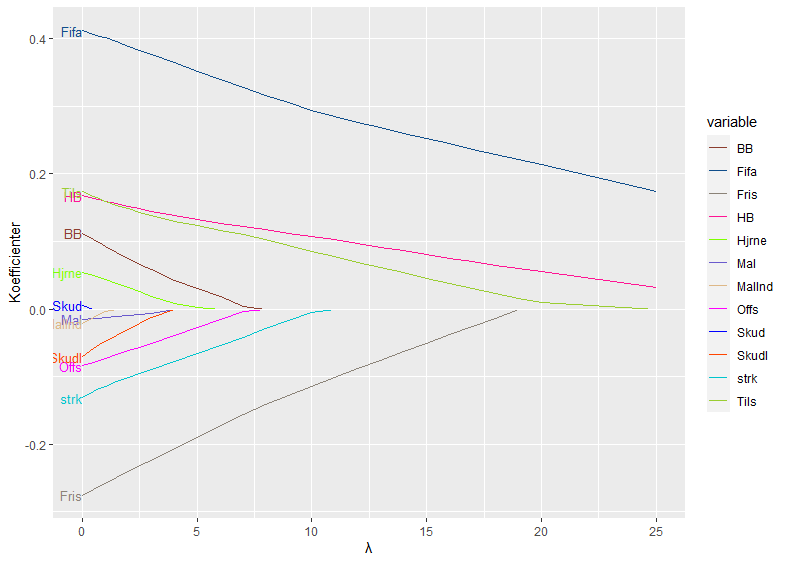
\includegraphics[width=\textwidth]{LINEPLOTDYNALPHA.png}
%    \caption{$\hat{\beta}^{\text{lasso}}$-koefficienter for forskellige straf-størrelser i den Dynamiske Rao Kupper Model med lasso-straf}
%    \label{fig:DBetaLasso}
%  \end{subfigure}
%  \begin{subfigure}[b]{\linewidth}
%    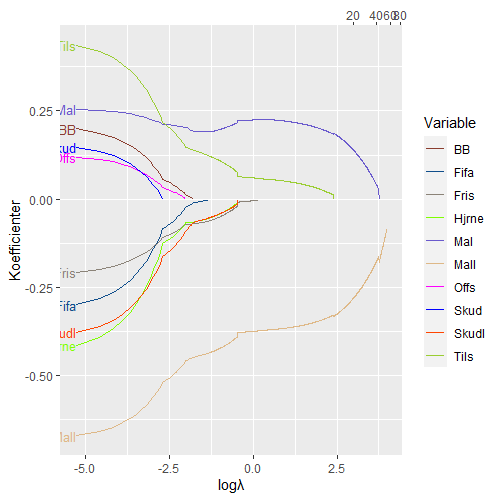
\includegraphics[width=\textwidth, height = 0.75 \textwidth]{SKLMSA.png}
%    \caption{$\hat{\beta}^{\text{lasso}}$-koefficienter for forskellige straf-størrelser i Rao Kupper Modellen med lasso-straf. Bemærk at første-aksen er logaritmetransformeret.}
%%    \label{fig:StatiskLine}
% \end{subfigure}
%\caption{\textit{Estimerede koefficienter mod $\lambda$-værdier for Rao Kupper modellen og Den Dynamiske model}}
%  \label{fig:KoefficienterLambda}
%\end{figure}
\\
\begin{figure}[h!]
    \centering
    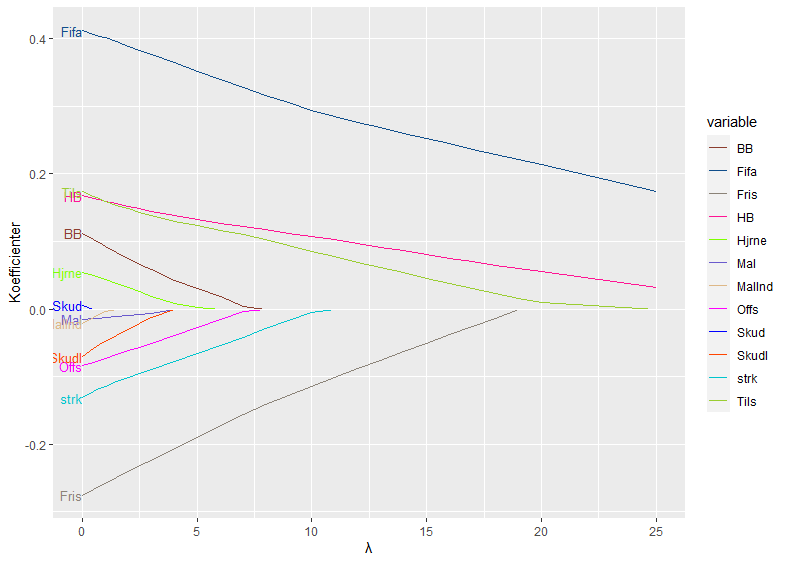
\includegraphics[width=\textwidth]{LINEPLOTDYNALPHA.png}
    \caption{\textit{$\hat{\beta}^{\text{lasso}}$-koefficienter mod $\lambda$ i den dynamiske model}}
    \label{fig:DBetaLasso}
\end{figure}
\begin{figure}[h!]
    \centering
    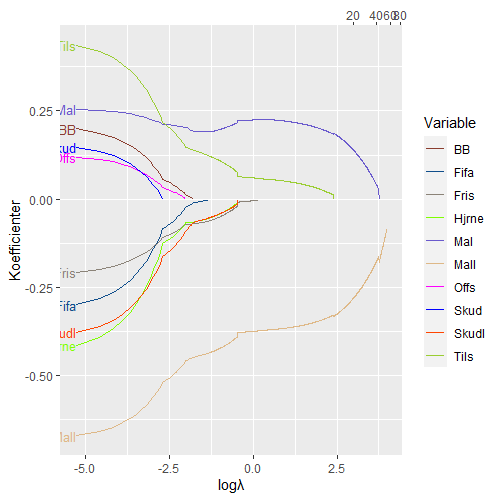
\includegraphics[width=0.75\textwidth,height=0.6\textwidth]{SKLMSA.png}
    \caption{\textit{$\hat{\beta}^{\text{lasso}}$-koefficienter mod $\log\lambda$ i Rao-Kupper}}
    \label{fig:SBetaLasso}
\end{figure}
\par  Eftersom målet er at minimalisere vores prædiktionsfejl, ønsker vi at identificere den $\lambda$, der minimerer dem, hvilket vi som nævnt gør ved brug af krydsvalidering. Vi har valgt at lave krydsvalidering på de 30 sidste runder af fodboldsæsonen 2015-2016, for at kunne at dele observationerne op i 6 lige store dele $(Q=6)$. Det vil sige, at vi forudsiger 5 runder (30 kampe) ad gangen. Inddelingerne af runderne er som følgende; $\{4,8\},\{9,13\},\{14,18\},\{19,23\},$ $\{24,28\},\{29,33\}$. Dette er gjort for begge modeller, for at kunne sammenligne deres prædiktionsfejl. For hver delmængde estimerer vi $\hat{\beta}^{\text{lasso}}$ med $\lambda \in [0,30]$ for den dynamiske model og $\lambda \in [0,6]$ for Rao-Kupper. $\lambda$-intervallerne er valgt ud fra Figur \ref{fig:DBetaLasso} \ref{fig:SBetaLasso}, med forventning om at alle parametre vil være fjernet ved slutningen af intervallet. Hver gang vi fjerner en parameter vil denne parameter forblive fjernet, og dermed ikke blive testet for de resterende $\lambda$'er. Figur (\ref{fig:Prædiktionsfejl}) viser plots af prædiktionsfejl, hvor hver linje på graferne repræsenterer prædiktionsfejlene for en kamp i forhold til $\lambda$. Hver $\lambda$ har altså 180 tilhørende prædiktionsfejl. På Figur (\ref{fig:DynMSPELine}) og (\ref{fig:DynLogLossLine}) ser vi, at variansen i prædiktionsfejlene er faldende når $\lambda$ stiger, hvilket også er forventeligt jvf. \textit{The Bias-Variance Decomposition}. Derudover er det også en naturlig følge idet $\lambda \rightarrow \infty \Rightarrow |\hat{\beta}| \rightarrow 0 \Rightarrow \pi_i \rightarrow \pi_j \Rightarrow \hat{p}_{i\cdot ij} \rightarrow \hat{p}_{j \cdot ij}$. Yderligere ser vi, at de største prædiktionsfejl mindskes når $\lambda$ stiger. De største prædiktionsfejl kommer fra kampe som er endt uafgjort og vores estimerede sandsynlighed for udfaldet uafgjort i de kampe er meget små. Som nævnt går holdenes styrker mod hinanden når $\lambda \rightarrow \infty$, hvilket også betyder at vores estimerede sandsynligheder for udfaldet uafgjort (for fast $\theta$) er størst når $\lambda \rightarrow \infty$, hvorfor de største prædiktionsfejl mindskes når $\lambda$ stiger. Samme sted som disse fejl slutter, ser vi også linjer som ikke ændrer sig meget i forhold til $\lambda$. Det er uafgjorte kampe for hold med styrker, som er tæt på hinanden - hvor der i forvejen er estimeret en høj sandsynlighed for udfaldet uafgjort.\par
 Vi ser udviklingen af prædiktionsfejlene for Rao-Kupper i Figur \ref{fig:MSPEStat} og \ref{fig:LogLossStat}. De ændrer sig stort set ikke når $\lambda$ stiger, hvilket følger den udvikling vi så i Figur \ref{fig:SBetaLasso}. Det tyder på at lasso-straffen, ikke har en lige så stor betydning for Rao-Kupper modellens prædiktionsevne, som den har i Den Dynamiske model. Dette underbygges yderligere af Figur (\ref{fig:Tabsfunktioner}), hvor vi ser at de gennemsnitlige prædiktionsfejl i den dynamiske model er mindst for $\lambda = 3$, hvorefter de stiger, og i Rao-Kupper ikke ændres meget. De er ikke uændret og vi ser, at de er mindst for $\lambda = 0.94$. Vi ser yderligere at for før lasso indføreres ($\lambda = 0$) har Rao-Kupper lavere prædiktionsfejl end den dynamiske model, men efter lasso har den dynamiske lavere prædiktionsfejl end Rao-Kupper. Tabel (\ref{tab:KVMSPELOGLOSS}) viser disse ændringer af prædiktionsfejl før og efter lasso, samt en \textit{baseline} som viser fejlene ved altid at gætte på de gennemsnitslige sandsynligheder for hjemmesejr, udesejr og uafgjort. \\
\begin{figure}[h!]
  \centering
  \begin{subfigure}[b]{0.45\textwidth}
    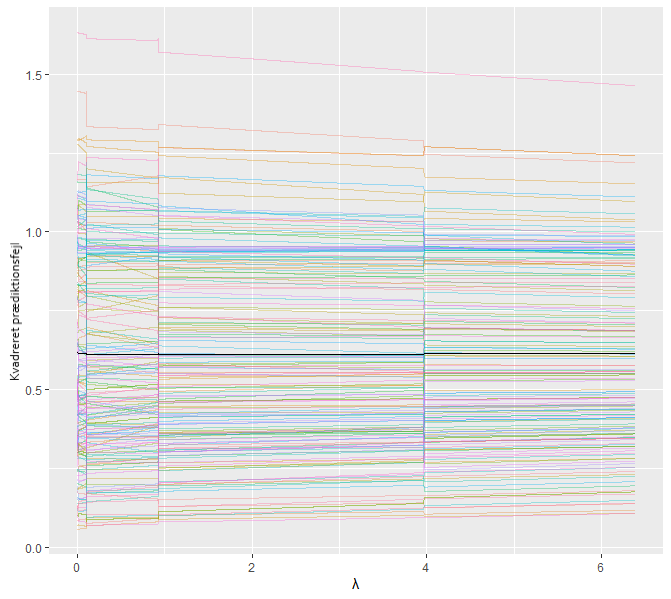
\includegraphics[width=\textwidth]{MSPESTATISK1.png}
    \caption{\textit{Kvadreret prædiktionsfejl mod $\lambda$ for Rao-Kupper}}
    \label{fig:MSPEStat}
  \end{subfigure}
    \hspace{0.2cm}
  \begin{subfigure}[b]{0.45\linewidth}
    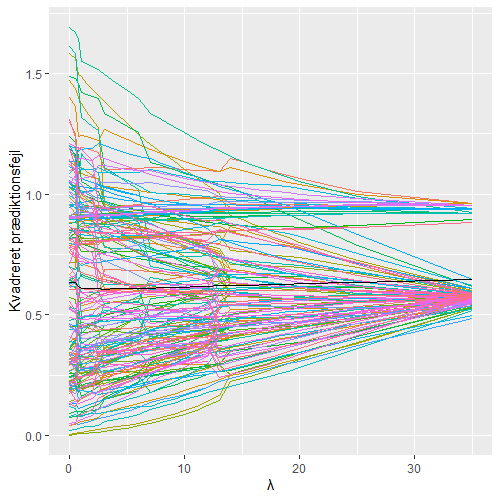
\includegraphics[width=\textwidth]{MSPELINEALPHA.png}
    \caption{\textit{Kvadreret prædiktionsfejl mod $\lambda$ for den dynamiske model}}
    \label{fig:DynMSPELine}
  \end{subfigure}
    \hspace{0.2cm}
    \begin{subfigure}[b]{0.45\textwidth}
    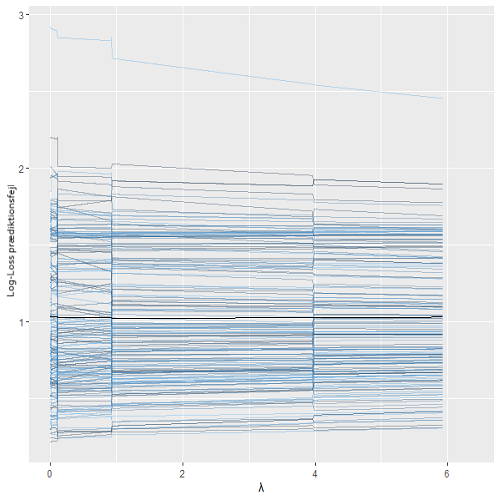
\includegraphics[width=\textwidth]{LOGLOSSSTATISK1.png}
    \caption{\textit{Log-prædiktionsfejl mod $\lambda$ for Rao-Kupper \textcolor{white}{modellen}}}
    \label{fig:LogLossStat}  
    \end{subfigure}
      \hspace{0.2cm}
  \begin{subfigure}[b]{0.45\linewidth}
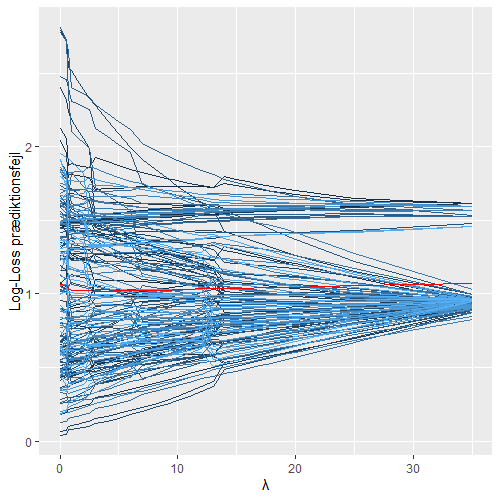
\includegraphics[width=\textwidth]{LINELOGLOSSALPHA.png}
    \caption{\textit{Log-prædiktionsfejl mod $\lambda$ for den dynamiske model}}
    \label{fig:DynLogLossLine}  
    \end{subfigure}
\caption{\textit{Prædiktionsfejl ved krydsvalidering. Hver linje repræsentere fejlene for en fodboldkamp mod $\lambda$. Gennemsnittet er vist med en sort linje med MSPE som tabsfunktion og med en rød linje med log loss som tabsfunktion.}}
  \label{fig:Prædiktionsfejl}
\end{figure}


\begin{figure}[h!]
  \centering
\begin{subfigure}[b]{0.45\textwidth}
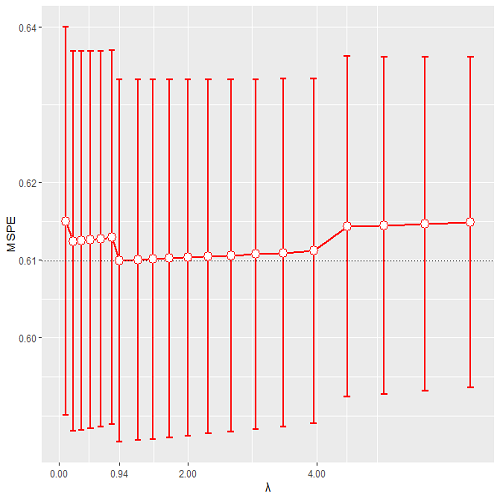
\includegraphics[width=\textwidth]{MSPEBARPLOTSTATNY1.png}
    \caption{\textit{MSPE mod $\lambda$ for Rao-Kupper}}
    \label{fig:MSPEBarStat}
  \end{subfigure}
  \hspace{0.2cm}
    \begin{subfigure}[b]{0.45\textwidth}
    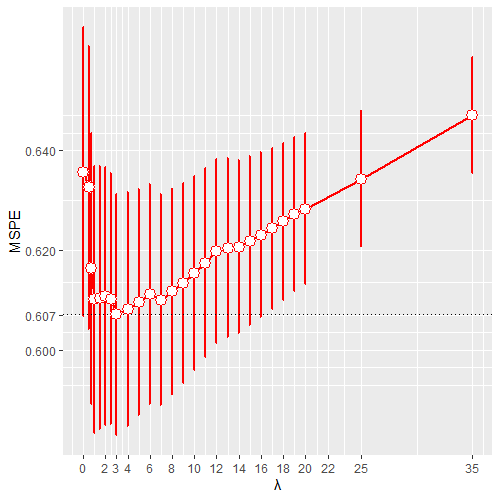
\includegraphics[width=\textwidth]{BARMSPENYALPHA.png}
    \caption{\textit{Log-Loss mod $\lambda$ for Rao-Kupper}}
    \label{fig:MSPEBarDyn}  
    \end{subfigure}
    \hspace{0.2cm}
  \begin{subfigure}[b]{0.45\linewidth}
    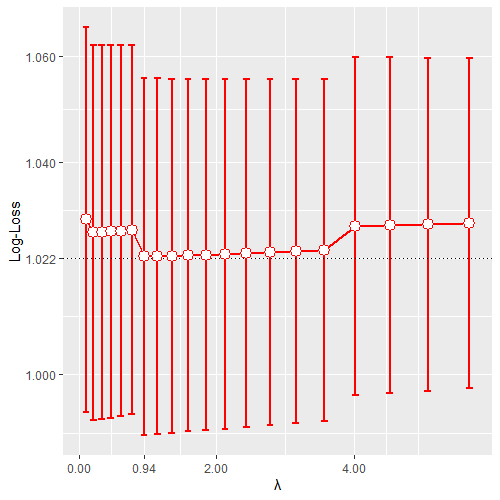
\includegraphics[width=\textwidth]{STATLOGLOSSBARNY1.png}
    \caption{\textit{Log-Loss mod $\lambda$ for Rao-Kupper}}
    \label{fig:LogLossBarStat}
  \end{subfigure}
  \hspace{0.2cm}
      \begin{subfigure}[b]{0.45\linewidth}
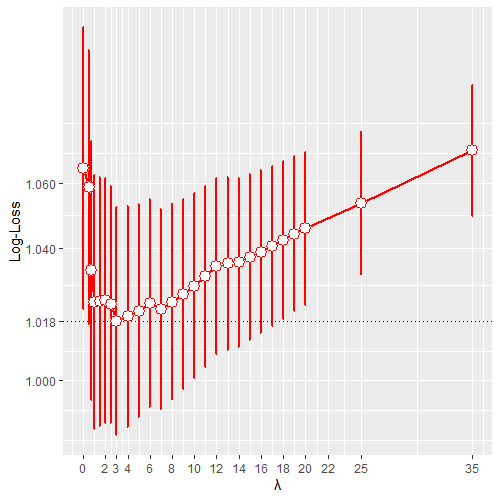
\includegraphics[width=\textwidth]{BARPLOTLOGALPHANY.png}
    \caption{\textit{Log-Loss mod $\lambda$ for den dynamiske model}}
    \label{fig:LogLossBarDyn}  
    \end{subfigure}
\caption{\textit{Plot af tabsfunktioner med tilhørende standardafvigelser mod $\lambda$ }}
  \label{fig:Tabsfunktioner}
\end{figure}


\begin{table}[ht]
\centering
\begin{adjustbox}{max width=\textwidth}
\begin{tabular}{|l|cc|}
\hline 
 & MSPE & Log-Loss  \\
 \hline
Baseline & 0.639 & 1.057 \\
Rao Kupper & 0.615 & 1.028 \\
Dynamisk & 0.636 & 1.064 \\
Rao Kupper Lasso ($\lambda=0.94$)& 0.611 & 1.022 \\
Dynamisk Lasso ($\lambda=3$) & 0.607 & 1.018 \\
   \hline   
\end{tabular} 
\end{adjustbox}
\caption{\label{tab:KVMSPELOGLOSS}\textit{Krydsvaliderings prædiktionsfejl for de to modeller med og uden lasso-straf, samt prædiktionsfejl for Baseline, som er lavet ud fra den konstante prædiktion $(\bar{Hjemmesejr},\bar{Udesjer}, \bar{Uafgjort}) = (0.456,0.322,0.222)$}}
\end{table}
\newpage
Tabel \ref{tab:EstKoefOptLambda} viser de estimerede koefficienter tilhørende Rao-Kupper og den dynamiske model, hvor $\lambda$ (valgt ved krydsvalidering) er henholdsvis $0.94$ og $3$. I Rao-Kupper er der fire  parametre numerisk større end 0, og i den dynamiske model er der 9. Standardfejlene for de bevarede parametre er ikke ændret meget, i forhold til hvad de var før lasso-straffen, og vi konkluderer derfor ikke noget nyt i forhold til deres signifikans. Vi ser, at parametrene BoldBesiddelse, Skud og SkudIndenfor er fjernet fra begge modeller. Det kunne tyde på, at disse parametre ikke har en stor korrelation med udfaldene eller, at de har en stor korrelation med andre parametre. Det er forventeligt, at både Skud og Skudindenfor vil være positivt korrelerede med hinanden, samt med MålScoret. \\
\begin{table}[ht!]
\centering
\begin{adjustbox}{max width=\textwidth}
\begin{tabular}{|l|rrrr|rrrr|}
\hline
\multicolumn{1}{|l|}{} & \multicolumn{4}{l|}{Rao Kupper Model} & \multicolumn{4}{l|}{Dynamisk Model} \\\hline 
Parameter & $\hat{\beta}^{\text{lasso}}$ & SE &2.5\%&97.5\%& $\hat{\beta}^{\text{lasso}}$ & SE&2.5\%&97.5\%\\
 \hline
HjemmeBaneFordel   & 0 & 0 & 0 & 0                 & 0.138  & 0.067 & 0.006 & 0.270\\
SejrStreak         & 0 & 0 & 0 & 0                 & -0.087 & 0.119 & -0.321 & 0.146\\
FifaRating         & 0 & 0 & 0 & 0                 & 0.359 & 0.146  & 0.073 & 0.646 \\
Hjørne             & 0 & 0 & 0 & 0                 & 0.035 & 0.100  & -0.160 & 0.230\\
OffSide            & 0 & 0 & 0 & 0                 & -0.015 & 0.099 & -0.210 & 0.179\\
MålScoret          & 0.224 & 0.196 & -0.160 & 0.608         & 0.017 & 0.112 & -0.203 & 0.236\\
MålLukketInd       & -0.380 & 0.162 & -0.698 & -0.062        & 0.083 & 0.114 & -0.141 & 0.307\\
Tilskuere          & 0.061 & 0.134 & -0.202 & 0.324         & 0.091 & 0.125 & -0.154 & 0.336\\
BoldBesiddelse     & 0 & 0 & 0 & 0                 & 0 & 0 & 0 & 0\\
Skud               & 0 & 0 & 0 & 0                 & 0 & 0 & 0 & 0  \\
SkudIndenfor       & 0 & 0 & 0 & 0                 & 0 & 0 & 0 & 0 \\
Frispark           & -0.005 & 0.130 & -0.260 & 0.250        & -0.190 & 0.097 & -0.380 & 0.000\\
$\theta$           & 1.662 & 0.120 & -1.427 & 1.897         & 1.643 & 0.119 & 1.411 & 1.876\\
   \hline   
\end{tabular} 
\end{adjustbox}
\caption{\label{tab:EstKoefOptLambda}\textit{Estimerede parametre for de to modeller fundet ved krydsvalidering}}
\end{table}\\
Ud fra tesen om, at bookmakerenes odds har en korrelation med vores estimerede sandsynligheder for udfaldene, opstiller vi en profitfunktion for en simpel betting strategi. Vi satser $\hat{p}_{i\cdot ij}(t)\mathcal{C}$ på sejr til hold $i$, $\hat{p}_{j\cdot ij}(t)\mathcal{C}$ på sejr til hold $j$ og $\hat{p}_{0\cdot ij}(t)\mathcal{C}$, hvor $\mathcal{C}$ betegner hvor mange penge vi satser på hver kamp. For at opstille profitten henter vi odds for hver af kampene. De odds vi måler op imod er gennemsnitlige odds fra diverse bookmakere, og er hentet fra Oddsportal.com \cite{Oddsportal}. Vi kalder oddsne for $odds_i(t),\; odds_j(t), \; odds_0(t)$, som henholdsvis repræsenterer odds for sejr til hold $i$, odds for sejr til hold $j$ og odds for uafgjort tilhørende en kamp mellem hold $i$ og hold $j$ i spillerunde $t$. Dermed bliver funktionen for den gennemsnitslige profit:
\begin{align}
    \overline{\text{Profit}}&= \frac{1}{N}\sum_t\sum_{i<j}\Big{[} \underbrace{\mathcal{C}\big{(}\hat{p}_{i\cdot ij}(t)odds_i(t)y_{i\cdot ij}(t)+\hat{p}_{j\cdot ij}(t)odds_j(t)y_{j\cdot ij}(t)+\hat{p}_{0\cdot ij}(t)odds_0(t)y_{0\cdot ij}(t)\big{)}}_{\text{Marginal Gevinst}} -\underbrace{\mathcal{C}}_{Omk}\Big{]},\label{func:Profit}
\end{align}
hvor den marginale gevinst er gevinsten ved oddsne placeret på kampen mellem hold $i$ og $j$ i spillerunde t, og $\mathcal{C}$, tolker vi som den marginale omkostning eller pris for at placere disse odds. \\I Figur \ref{fig:OddsPlot} har vi taget de inverse af vores sandsynligheder for at sammenligne med bookmakernes udbudte odds fordelt på hjemmebanesejr, udebanesejr og uafgjort. Vi bruger dem som benchmark, men det skal tages in mente, at bookmakernes odds konverteret til sandsynligheder summerer over 1. Derudover er det også klart, at bookmakerne for at mindske risiko, justerer deres odds løbende i forhold til hvor store beløb der er placeret på de forskellige odds. For lave fittede værdier minder begge modellers estimerede odds, om bookmakernes odds, men for høje værdier stiger variansen. Vi ser en klar tendens til forøget varians ved høje fittede værdier. Derudover er det bemærkelsesværdigt, at for ikke-uafgjorte tyder det på at middelværdierne er ens for bookmakernes odds og de estimerede odds. Men for uafgjorte kampe, er der en klar tendens til at vores estimerede odds er højere end bookmakernes. Vi ser, at vores estimerede odds for uafgjort aldrig går under 4. Det skyldes, at vi har en øvre grænse for den estimerede sandsynlighed for uafgjort (når to hold er lige gode), som er bestemt af $\theta$. For $\theta$ som hendholdsvis for Rao-kupper og den dynamiske model er 1.662 og 1.643, bliver de respektive nedre grænser for estimerede odds 4.021 og 4.110. Da bookmakernes sandsynligheder ikke summer til 1, er det klart at der vil være en forskel i middelværdier samlet set.   

\begin{figure}[ht!]
  \centering
  \begin{subfigure}[b]{0.4\textwidth}
    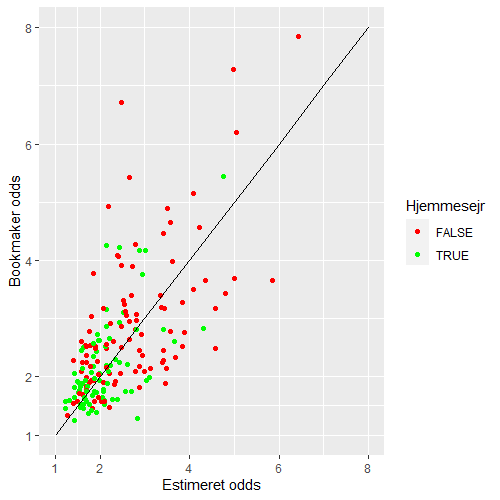
\includegraphics[width=\textwidth]{DynHjemmeOdds.png}
    \caption{\textit{Dynamisk estimerede odds for hjemme mod bookmaker odds}}
    \label{fig:DynHjemmeOdds}
  \end{subfigure}
    \hspace{0.2cm}
    \begin{subfigure}[b]{0.4\linewidth}
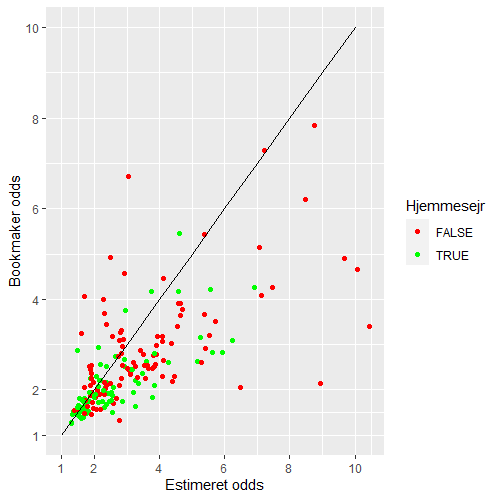
\includegraphics[width=\textwidth]{StatiskHjemmeOdds.png}
    \caption{\textit{Rao Kupper estimerede odds for hjemme mod bookmaker odds}}
    \label{fig:StatHjemmeOdds}  
    \end{subfigure}
  \hspace{0.2cm}
  \begin{subfigure}[b]{0.4\linewidth}
    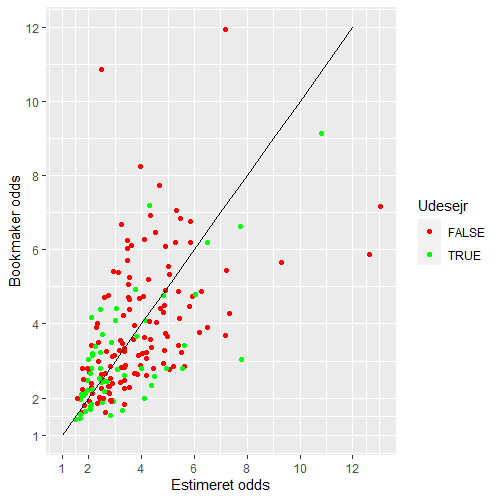
\includegraphics[width=\textwidth]{DynUdeOdds.png}
    \caption{\textit{Dynamisk estimerede odds for ude mod bookmaker odds}}
    \label{fig:DynUdeOdds}
  \end{subfigure}
        \hspace{0.2cm}
  \begin{subfigure}[b]{0.4\linewidth}
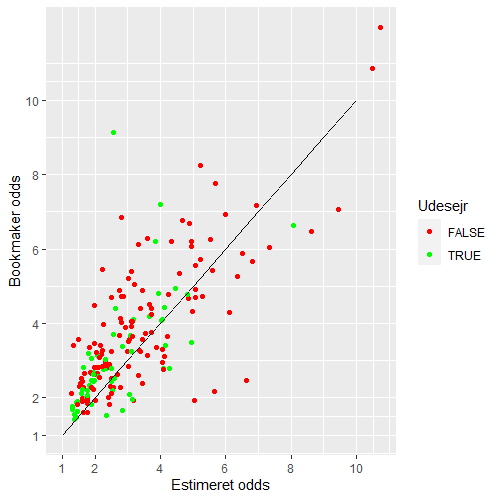
\includegraphics[width=\textwidth]{StatUdeOdds.png}
    \caption{\textit{Rao Kupper estimerede odds for ude mod bookmaker odds}}
    \label{fig:StatUdeOdds}  
    \end{subfigure}
    \hspace{0.2cm}
    \begin{subfigure}[b]{0.4\textwidth}
    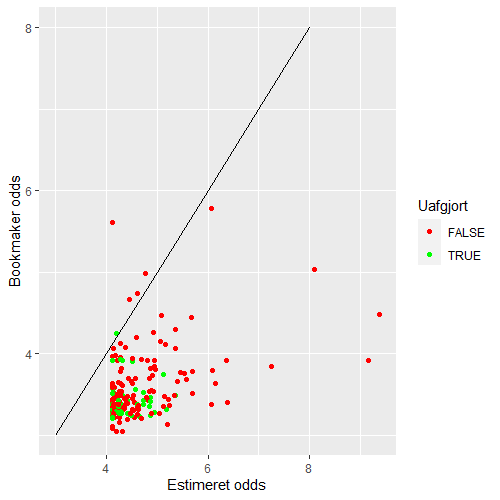
\includegraphics[width=\textwidth]{DynUafgjortOdds.png}
    \caption{\textit{Dynamisk estimerede odds for uafgjort mod bookmaker odds}}
    \label{fig:DynUafgjortOdds}  
    \end{subfigure}
          \hspace{0.2cm}
  \begin{subfigure}[b]{0.4\linewidth}
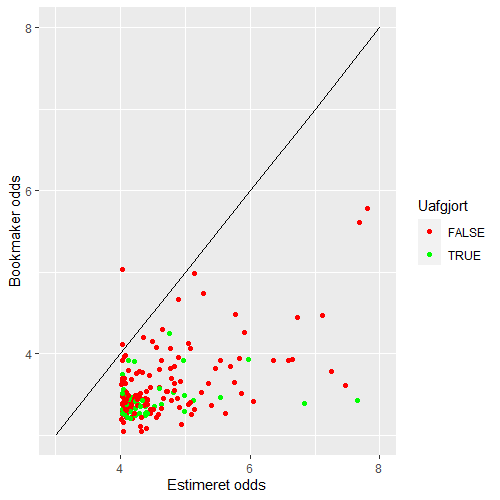
\includegraphics[width=\textwidth]{StatUafgjortOdds.png}
    \caption{\textit{Rao Kupper estimerede odds for uafgjort mod bookmaker odds}}
    \label{fig:StatUafgjortOdds}  
    \end{subfigure}
\caption{\textit{Plots af estimerede odds mod bookmaker odds, for hjemmesejr, udesejr og uafgjort. Den sorte streg indikerer hvor de estimerede odds er lig bookmakernes odds. De estimerede odds er beregnet som de inverse sandsynligheder.}}
  \label{fig:OddsPlot}
\end{figure}
\clearpage
Til at undersøge hvordan de to modeller med og uden lasso-straf præsterer på ukendt data, har vi valgt at teste dem på Superligaen for sæson 2014-2015, hvor vi starter fra 3. spillerunde. Vi måler dem igen op i mod hinanden med MSPE og Log-Loss prædiktionsfejl. Resultatet af undersøgelsen ses i Tabel \ref{tab:Test2014}. Vi ser at lasso i begge tilfælde forbedrer modellernes prædiktionsevne. Forbedring ses at være størst i Rao-Kupper, hvor prædtiktionsfejlen bliver mindskes med cirka 14\%.  Vi ser også, at den dynamiske model opnår den ben bedste prædiktionsevne både før og efter. Faktisk er den dynamiske uden lasso bedre end Rao-Kupper med lasso. Begge modeller ses, at være markant bedre end baseline modellen efter lasso.  
\begin{table}[thb!]
\centering
\begin{adjustbox}{max width=\textwidth}
\begin{tabular}{|l|ccc|}
\hline 
Model & MSPE & Log-Loss & \overline{Profit} \\
 \hline
Baseline & 0.649 & 1.074 & -0.067\\
Rao Kupper Model & 0.720 & 1.191 & -0.057\\
Dynamisk Model & 0.613 & 1.027 & -0.022\\
Rao Kupper Model ($\lambda = 0.94$) & 0.618 & 1.030 & -0.034\\
Dynamisk Model ($\lambda = 3$) & 0.603 & 1.012 & -0.023 \\
   \hline   
\end{tabular} 
\end{adjustbox}
\caption{\label{tab:Test2014}
\textit{Prædiktionsfejl ved test af modellerne på data fra 2014-2015. De estimerede koefficienter for modellerne med lasso-straf ses i Tabel (\ref{tab:EstKoefOptLambda}). Profitten er udregnet fra profitfunktionen (ligning \ref{func:Profit}) med \mathcal{C}=1 }}
\end{table}\\

\clearpage
\section{Diskussion}
Vi har i projektet vist hvorpå Bradley-Terry modellen kan udvides til Rao-Kupper modellen, samt hvordan denne kan implementeres til både at rangere ud fra parvise sammenligninger, samt forudsige udfald af af parvise sammenligninger. Derudover har vi vist, hvordan lasso kan bruges til træffe parameterudvælgelse i modellen. Vi har implementeret modellen i praksis og valgt at teste den af på rangering af fodboldhold og prædiktion af udfald af fodboldkampe. Der er selvfølgelig forskellige måder at implementere modellen på, samt et utal af muligheder for, hvor modellen kan anvendes i praksis. Vi har i projektet "kun" anvendt op til 12 parametre. I et fremtidigt projekt, kunne det være spændende at indkludere endnu flere, for sandsynligvis at se en større forbedring ved lasso.\par
Til at estimere parametrene i den dynamiske model valgte vi at sætte $\alpha=3$, eftersom det gav den største likelihoodværdi i vores insample test. Eftersom vi har valgt $\alpha$-værdien ved at sammenligne fits af modellen på 2015, har vi ikke noget belæg for at den værdi vil passe godt på ukendt data. En anden og måske bedre metode til at udvælge denne $\alpha$-værdi, ville være ved krydsvalidering, ligesom vi har valgt $\lambda$. Ydermere kunne der testes på flere års data, for at få et mere generelt billede af hvordan den influerer modellen. I det hele taget ville det være interessant at estimere den Dynamiske models parametre ud fra flere års data, især når den skal bruges til forudsige udfald på ukendt data. Det samme gælder for Rao-Kupper, hvis man gerne vil få et indblik i hvilke kovariater der influerer på rangeringen generelt. Hvorimod hvis det eneste der ønskes med Rao Kupper modellen, er at rangere hold eller produkter, kan man med fordel estimere styrkerne uden brug af kovariater med udgangspunkt i ligning (\ref{func:LikelihoodUdenBeta}). \textcolor{blue}{Ved at estimere styrkerne ved den metode, vil man også mindske risikoen for Type I og II fejl, eftersom der vil være færre parametre at teste.} \\ \newline 
Fodboldhold er ikke det mest interessante at rangere, eftersom der allerede findes et regelsæt der bestemmer hvilke hold der er bedst rangeret, men tilgengæld giver det også et meget godt benchmark for hvordan modellernes evne til at rangere er. Vi så i Tabel \ref{tab:Styrkeestimater} at Rao-Kupper rangerer holdene bedst, når vi måler dem op imod den endelige stilling i Superligaen. Derimod så vi i Tabel (\ref{tab:KVMSPELOGLOSS}) og (\ref{tab:Test2014}) at den dynamiske model opnår mindre prædiktionsfejl i krydsvalideringen samt i prædiktionen på data fra Superligaen i sæson 2014-2015.\\
På trods af at vi har fokuseret anvendelsen af disse modeller på fodboldhold, er der ikke nogen teoretisk forskel på om det er fodboldhold, vin, charter rejser eller noget helt fjerde der skal rangeres. Der vil selvfølgelig være forskel på, hvor tilgængeligt data til sådanne parvise sammenligninger er. I nogle produktkategorier har tid også en stor betydning, eksempelvis kan man forestille sig, at der er forskel på forbrugerpræferencer af drikkevarer alt efter sæsonen, som giver anledning til at bruge $\alpha$-parameteren, til at fange de trends der kan være i markedet. På samme vis, som vi opdelte sæsonen i spillerunder, kan en anden tilsvarende tidsopdeling være af et år, som gør det muligt at rangere et produkt ud fra forbrugernes præferencer de seneste uger/måneder, fremfor at tage udgangspunkt i hele det sidste år. \\\\
Rao-kupper modellen kan ligeledes anvendes til at rangere produkter ud fra forbrugerpræferencer ved parvise sammenligninger.  
Her kan profitfunktionen bruges i en situation med en producent, hvor producenten estimerer sandsynligheden for at forbrugergruppen køber hvert af hans/hendes produkter, og derefter producerer en tilsvarende mængde af hvert produkt. Produkterne kan her, ligesom kampe har odds, have forskellige dækningsbidrag, og med udgangspunkt i sandsynligheder kontra dækningsbidrag, kan producenten optimere sin forventede profit. \\
\# Kunne være interresandt at teste Rao-Kuppers rangerings evne før og efter lasso.
\# Vores Rangerings model  Rao-Kupper viser at Mal skoret og Mål lukket ind, er gode variable til at beskrive den endelig rangering af fodboldhold ved slutningen af en sæson. Dette kommer nok ikke som nogen overraskelse for nogle. Men hvis det var sammenlinging af produkter kunne det være vanskeligere at identificere disse problemer. \# skodsætning.
\section{Konklusion}


Vi har i opgaven vist, hvordan Rao-Kupper modellen kan bruges til at rangere ud fra parvise sammenligninger, samt hvordan modellen kan bruges til at forudsige udfald af parvise sammenligninger. Vi har udviklet og implementeret kode til at gøre dette i praksis og forbedret modellens prædiktionsevne ved brug af lasso-metoden. Vi har testet modellen til rangering af fodboldhold i den danske Superliga - resultatet er forskelligt fra den faktisk rangering ved 3-1-0 pointsystemet, men kommer tæt på. Det betyder ikke at resultatet er forkert. Det er blot en anden måde at rangere på. Derudover har vi testet modellens prædiktionsevne på udfald af fodboldkampe i den danske Superliga og vist lasso-metoden kan bruges til at forbedre denne. Derudover har vi vist, at vi ikke forkaster signifikans af parametrene hjemmebane fordel og Fifa-ratings når det gælder forudsigelse af kampes udfald ved et signifikansniveau på 5\%. 
\\


\sout{De to metoder vi har valgt at anvende Rao Kupper modellen på, viste sig som forventet at have hver deres anvendelsesområde. Vores anvendelse af Rao Kupper modellen er bedst til at rangere holdene, hvor den Dynamiske model er bedst til at estimere punktsandsynligheder for udfald. Begge modeller blev ud fra tabsfunktionerne forbedret med lasso, men den Dynamiske model fik den største forbedring. Hvorvidt denne forbedring viser sig at være signifikant, kan vi ikke konkludere eftersom }
\clearpage
\section{Litteraturliste}
Litteraturliste
\clearpage
\section{Appendiks}

\clearpage
\printbibliography %Printer referencer
\section{Ordforklaringer}
\end{document}
%\begin{figure}[h!]
%  \centering
%  \begin{subfigure}[b]{0.425\linewidth}
%    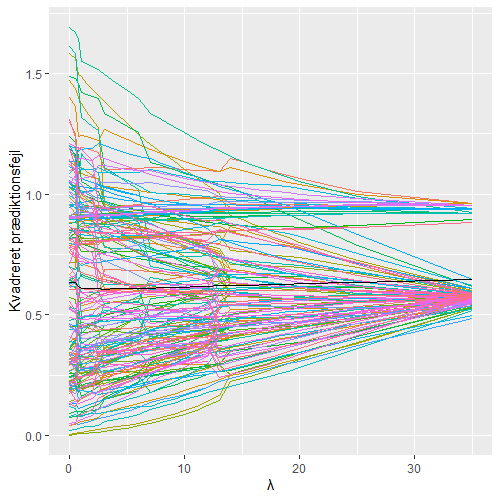
\includegraphics[width=\textwidth]{MSPELINEALPHA.png}
%    \caption{Kvadreret prædiktionsfejl mod $\lambda$ for den Dynamiske model med lasso-straf, hvor hver linje viser fejlene tilhørende én kamp, og den sorte linje viser gennemsnittet af fejlene, %altså MSPE}
%    \label{fig:DynMSPELine}
%  \end{subfigure}
%     \hspace{0.2cm}
%%  \begin{subfigure}[b]{0.425\linewidth}
% 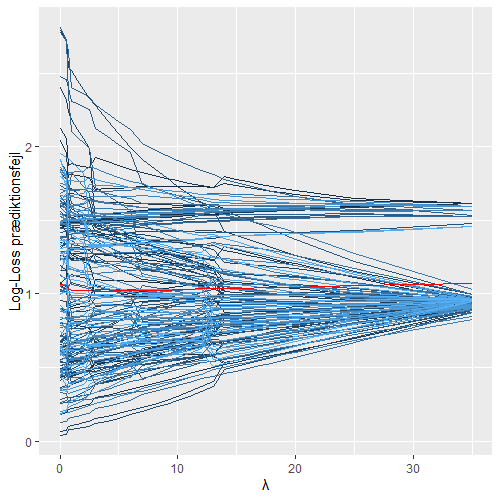
\includegraphics[width=\textwidth]{LINELOGLOSSALPHA.png}
 %   \caption{Log-prædiktionsfejl mod $\lambda$ for den dynamiske model med lasso-straf, hvor hver linje viser fejlene tilhørende én kamp, og den røde linje viser gennemsnittet af fejlene}
 %   \label{fig:DynLogLossLine}  
 %   \end{subfigure}
 %%   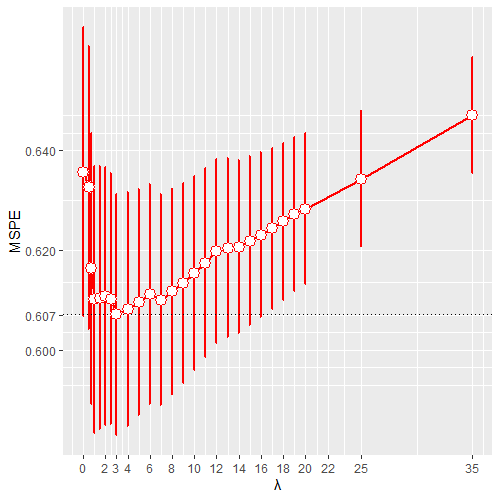
\includegraphics[width=\textwidth]{BARMSPENYALPHA.png}
 %   \caption{Zoomet ind på den sorte linje i ovenstående figur, viser altså MSPE for hver $\lambda$. Hver ende på barene er en standardfejl fra MSPE'en for den Dynamiske model med lasso-straf}
 %   \label{fig:MSPEBarDyn}
 % \end{subfigure}
 %     \hspace{0.2cm}
 %   \begin{subfigure}[b]{0.425\linewidth}
 %   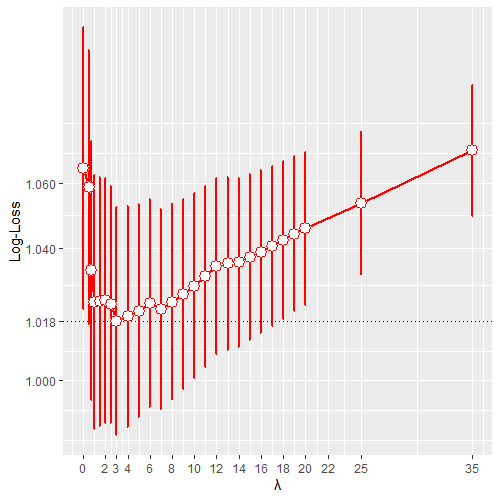
\includegraphics[width=\textwidth]{BARPLOTLOGALPHANY.png}
 %   \caption{Zoomet ind på den røde linje i ovenstående figur, viser altså gennemsnitlig Log-Loss for hver $\lambda$. Hver ende på barene er en standardfejl fra gennemsnittet for den Dynamiske model %med lasso-straf}
 %   \label{fig:LogLossBarDyn}    
 %   \end{subfigure}
%\%caption{\textit{MSPE og Log-Loss prædiktionsfejl fra Kryds-Validering i den Dynamiske Model}}
%  \label{fig:MSPELOGLOSDYN}
%\end{figure}

%FIGUR TIL STATISK RAO KUPPER
%\begin{figure}[htb!]
%  \centering
%  \begin{subfigure}[b]{0.4\textwidth}
%    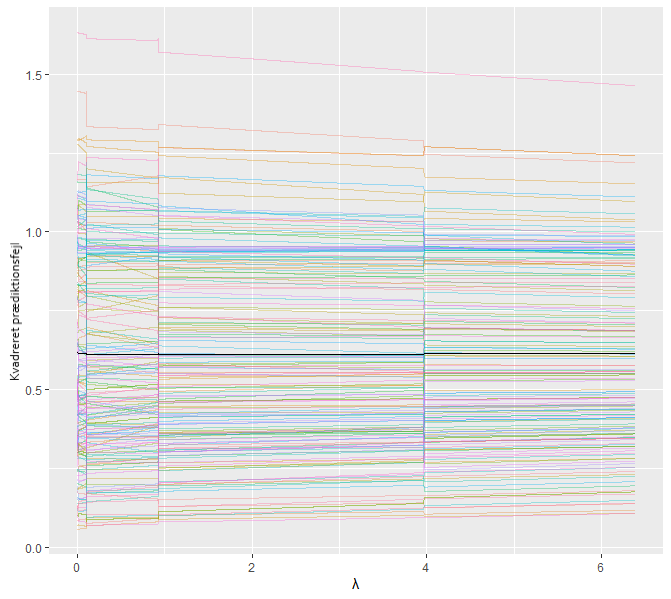
\includegraphics[width=\textwidth]{MSPESTATISK1.png}
%    \caption{Kvadreret prædiktionsfejl mod $\lambda$ for Rao Kupper modellen med lasso-straf, hvor hver linje viser fejlene tilhørende én kamp, og den sorte linje viser gennemsnittet af fejlene, altså MSPE}
%    \label{fig:MSPEStat}
%  \end{subfigure}
%  \hspace{0.2cm}
%  \begin{subfigure}[b]{0.4\textwidth}
%    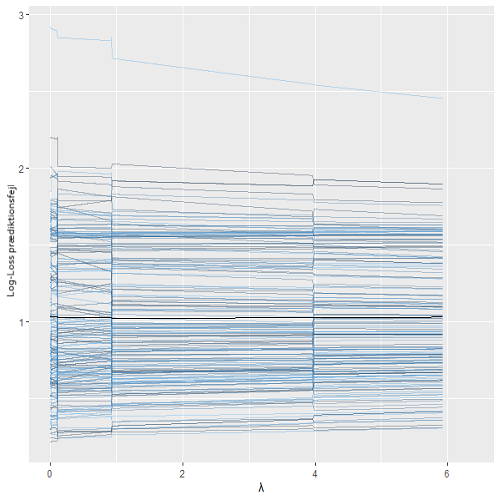
\includegraphics[width=\textwidth]{LOGLOSSSTATISK1.png}
%    \caption{Log-prædiktionsfejl mod $\lambda$ for Rao Kupper modellen med lasso-straf, hvor hver linje viser fejlene tilhørende én kamp, og den sorte linje viser gennemsnittet af fejlene}
%    \label{fig:LogLossStat}  
%    \end{subfigure}
%  \begin{subfigure}[b]{0.4\textwidth}
%    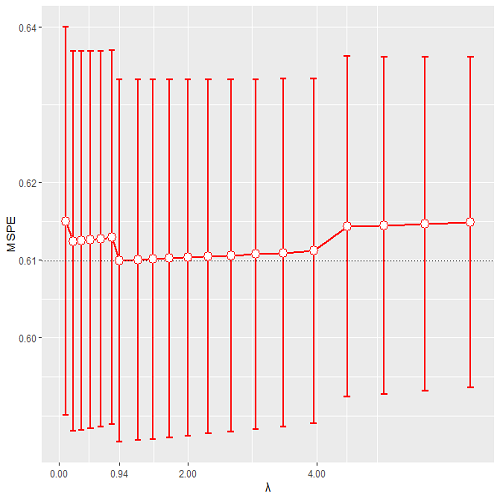
\includegraphics[width=\textwidth]{MSPEBARPLOTSTATNY1.png}
%    \caption{Zoomet ind på den sorte linje i ovenstående figur, viser altså MSPE for hver  $\lambda$. Hver ende på barene viser en standardfejl for MSPE'en fra Rao Kupper          modellen med %lasso-straf}
%    \label{fig:MSPEBarStat}
%  \end{subfigure}
%      \hspace{0.2cm}
%    \begin{subfigure}[b]{0.4\textwidth}
%    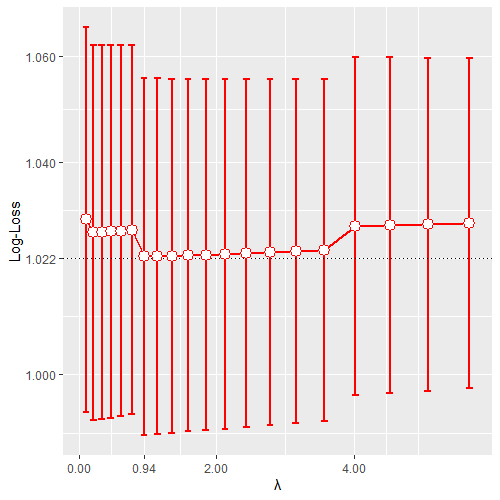
\includegraphics[width=\textwidth]{STATLOGLOSSBARNY1.png}
%   \caption{Zoomet ind på den røde linje i ovenstående figur, viser altså gennemsnitlig Log-Loss for hver $\lambda$. Hver ende på barene er en standardfejl fra gennemsnittet for Rao Kupper modellen %med lasso-straf}
%    \label{fig:LogLossBarStat}  
%    \end{subfigure}
%\caption{\textit{MSPE og Log-Loss fra Kryds-Validering i Rao Kupper Modellen}}
%\label{fig:MSPELOGLOSSStatisk}
%\end{figure}